\documentclass[
  stu,
  floatsintext,
  longtable,
  a4paper,
  nolmodern,
  notxfonts,
  notimes,
  colorlinks=true,linkcolor=blue,citecolor=blue,urlcolor=blue]{apa7}

\usepackage{amsmath}
\usepackage{amssymb}



\usepackage[bidi=default]{babel}
\babelprovide[main,import]{spanish}
\StartBabelCommands{spanish}{captions} [unicode, fontenc=TU EU1 EU2, charset=utf8] \SetString{\keywordname}{Palabras
Claves}
\EndBabelCommands


% get rid of language-specific shorthands (see #6817):
\let\LanguageShortHands\languageshorthands
\def\languageshorthands#1{}

\RequirePackage{longtable}
\RequirePackage{threeparttablex}

\makeatletter
\renewcommand{\paragraph}{\@startsection{paragraph}{4}{\parindent}%
	{0\baselineskip \@plus 0.2ex \@minus 0.2ex}%
	{-.5em}%
	{\normalfont\normalsize\bfseries\typesectitle}}

\renewcommand{\subparagraph}[1]{\@startsection{subparagraph}{5}{0.5em}%
	{0\baselineskip \@plus 0.2ex \@minus 0.2ex}%
	{-\z@\relax}%
	{\normalfont\normalsize\bfseries\itshape\hspace{\parindent}{#1}\textit{\addperi}}{\relax}}
\makeatother




\usepackage{longtable, booktabs, multirow, multicol, colortbl, hhline, caption, array, float, xpatch}
\usepackage{subcaption}
\renewcommand\thesubfigure{\Alph{subfigure}}
\setcounter{topnumber}{2}
\setcounter{bottomnumber}{2}
\setcounter{totalnumber}{4}
\renewcommand{\topfraction}{0.85}
\renewcommand{\bottomfraction}{0.85}
\renewcommand{\textfraction}{0.15}
\renewcommand{\floatpagefraction}{0.7}

\usepackage{tcolorbox}
\tcbuselibrary{listings,theorems, breakable, skins}
\usepackage{fontawesome5}

\definecolor{quarto-callout-color}{HTML}{909090}
\definecolor{quarto-callout-note-color}{HTML}{0758E5}
\definecolor{quarto-callout-important-color}{HTML}{CC1914}
\definecolor{quarto-callout-warning-color}{HTML}{EB9113}
\definecolor{quarto-callout-tip-color}{HTML}{00A047}
\definecolor{quarto-callout-caution-color}{HTML}{FC5300}
\definecolor{quarto-callout-color-frame}{HTML}{ACACAC}
\definecolor{quarto-callout-note-color-frame}{HTML}{4582EC}
\definecolor{quarto-callout-important-color-frame}{HTML}{D9534F}
\definecolor{quarto-callout-warning-color-frame}{HTML}{F0AD4E}
\definecolor{quarto-callout-tip-color-frame}{HTML}{02B875}
\definecolor{quarto-callout-caution-color-frame}{HTML}{FD7E14}

%\newlength\Oldarrayrulewidth
%\newlength\Oldtabcolsep


\usepackage{hyperref}




\providecommand{\tightlist}{%
  \setlength{\itemsep}{0pt}\setlength{\parskip}{0pt}}
\usepackage{longtable,booktabs,array}
\usepackage{calc} % for calculating minipage widths
% Correct order of tables after \paragraph or \subparagraph
\usepackage{etoolbox}
\makeatletter
\patchcmd\longtable{\par}{\if@noskipsec\mbox{}\fi\par}{}{}
\makeatother
% Allow footnotes in longtable head/foot
\IfFileExists{footnotehyper.sty}{\usepackage{footnotehyper}}{\usepackage{footnote}}
\makesavenoteenv{longtable}

\usepackage{graphicx}
\makeatletter
\newsavebox\pandoc@box
\newcommand*\pandocbounded[1]{% scales image to fit in text height/width
  \sbox\pandoc@box{#1}%
  \Gscale@div\@tempa{\textheight}{\dimexpr\ht\pandoc@box+\dp\pandoc@box\relax}%
  \Gscale@div\@tempb{\linewidth}{\wd\pandoc@box}%
  \ifdim\@tempb\p@<\@tempa\p@\let\@tempa\@tempb\fi% select the smaller of both
  \ifdim\@tempa\p@<\p@\scalebox{\@tempa}{\usebox\pandoc@box}%
  \else\usebox{\pandoc@box}%
  \fi%
}
% Set default figure placement to htbp
\def\fps@figure{htbp}
\makeatother


% definitions for citeproc citations
\NewDocumentCommand\citeproctext{}{}
\NewDocumentCommand\citeproc{mm}{%
  \begingroup\def\citeproctext{#2}\cite{#1}\endgroup}
\makeatletter
 % allow citations to break across lines
 \let\@cite@ofmt\@firstofone
 % avoid brackets around text for \cite:
 \def\@biblabel#1{}
 \def\@cite#1#2{{#1\if@tempswa , #2\fi}}
\makeatother
\newlength{\cslhangindent}
\setlength{\cslhangindent}{1.5em}
\newlength{\csllabelwidth}
\setlength{\csllabelwidth}{3em}
\newenvironment{CSLReferences}[2] % #1 hanging-indent, #2 entry-spacing
 {\begin{list}{}{%
  \setlength{\itemindent}{0pt}
  \setlength{\leftmargin}{0pt}
  \setlength{\parsep}{0pt}
  % turn on hanging indent if param 1 is 1
  \ifodd #1
   \setlength{\leftmargin}{\cslhangindent}
   \setlength{\itemindent}{-1\cslhangindent}
  \fi
  % set entry spacing
  \setlength{\itemsep}{#2\baselineskip}}}
 {\end{list}}
\usepackage{calc}
\newcommand{\CSLBlock}[1]{\hfill\break\parbox[t]{\linewidth}{\strut\ignorespaces#1\strut}}
\newcommand{\CSLLeftMargin}[1]{\parbox[t]{\csllabelwidth}{\strut#1\strut}}
\newcommand{\CSLRightInline}[1]{\parbox[t]{\linewidth - \csllabelwidth}{\strut#1\strut}}
\newcommand{\CSLIndent}[1]{\hspace{\cslhangindent}#1}





\usepackage{newtx}

\defaultfontfeatures{Scale=MatchLowercase}
\defaultfontfeatures[\rmfamily]{Ligatures=TeX,Scale=1}





\title{Proporcionalidad de Magnitudes}


\shorttitle{Proporcionalidad de Magnitudes}


\usepackage{etoolbox}


\course{Matemáticas Aplicadas a la Comunicación}

\ccoppy{\textcopyright~2025}



\author{Edison Achalma}



\affiliation{
{Escuela Profesional de Economía, Universidad Nacional de San Cristóbal
de Huamanga}}




\leftheader{Achalma}

\date{2025-05-20}


\abstract{Este trabajo explora los fundamentos matemáticos de la
proporcionalidad y sus aplicaciones en el campo de las Ciencias de la
Comunicación. Se analizan conceptos clave como razones, proporciones y
magnitudes, junto con sus implementaciones prácticas en estrategias
mediáticas, análisis de audiencias y diseño de mensajes. El estudio
demuestra cómo estas herramientas matemáticas optimizan procesos
comunicacionales en entornos digitales y tradicionales }

\keywords{proporcionalidad, comunicación, matemáticas
aplicadas, análisis de audiencias, estrategias mediáticas}

\authornote{\par{\addORCIDlink{Edison Achalma}{0000-0001-6996-3364}} 
\par{ }
\par{   El autor no tiene conflictos de interés que revelar.  Expreso mi
sincero agradecimiento a todas las personas que contribuyeron directa e
indirectamente a la realización de esta monografía. En especial. A mi
profesor, por su valiosa orientación, correcciones y sugerencias que
permitieron estructurar y mejorar este trabajo. A la institución
educativa y a la Facultad de Ciencias de la Comunicación, por brindar
las herramientas necesarias para mi desarrollo profesional. A los
autores y especialistas cuyas investigaciones sirvieron como base
teórica para este estudio. A mi familia y seres queridos, por su
constante apoyo emocional durante este proceso. Este trabajo es el
resultado de un esfuerzo colectivo, y por ello, mi más profundo
reconocimiento a quienes hicieron posible su culminación.  Los roles de
autor se clasificaron utilizando la taxonomía de roles de colaborador
(CRediT; https://credit.niso.org/) de la siguiente manera:  Edison
Achalma:   conceptualización, redacción}
\par{La correspondencia relativa a este artículo debe dirigirse a Edison
Achalma, Email: \href{mailto:elmer.achalma.09@unsch.edu.pe}{elmer.achalma.09@unsch.edu.pe}}
}

\makeatletter
\let\endoldlt\endlongtable
\def\endlongtable{
\hline
\endoldlt
}
\makeatother

\urlstyle{same}



\makeatletter
\@ifpackageloaded{caption}{}{\usepackage{caption}}
\AtBeginDocument{%
\ifdefined\contentsname
  \renewcommand*\contentsname{Tabla de contenidos}
\else
  \newcommand\contentsname{Tabla de contenidos}
\fi
\ifdefined\listfigurename
  \renewcommand*\listfigurename{Listado de Figuras}
\else
  \newcommand\listfigurename{Listado de Figuras}
\fi
\ifdefined\listtablename
  \renewcommand*\listtablename{Listado de Tablas}
\else
  \newcommand\listtablename{Listado de Tablas}
\fi
\ifdefined\figurename
  \renewcommand*\figurename{Figura}
\else
  \newcommand\figurename{Figura}
\fi
\ifdefined\tablename
  \renewcommand*\tablename{Tabla}
\else
  \newcommand\tablename{Tabla}
\fi
}
\@ifpackageloaded{float}{}{\usepackage{float}}
\floatstyle{ruled}
\@ifundefined{c@chapter}{\newfloat{codelisting}{h}{lop}}{\newfloat{codelisting}{h}{lop}[chapter]}
\floatname{codelisting}{Listado}
\newcommand*\listoflistings{\listof{codelisting}{Listado de Listados}}
\makeatother
\makeatletter
\makeatother
\makeatletter
\@ifpackageloaded{caption}{}{\usepackage{caption}}
\@ifpackageloaded{subcaption}{}{\usepackage{subcaption}}
\makeatother

% From https://tex.stackexchange.com/a/645996/211326
%%% apa7 doesn't want to add appendix section titles in the toc
%%% let's make it do it
\makeatletter
\xpatchcmd{\appendix}
  {\par}
  {\addcontentsline{toc}{section}{\@currentlabelname}\par}
  {}{}
\makeatother

%% Disable longtable counter
%% https://tex.stackexchange.com/a/248395/211326

\usepackage{etoolbox}

\makeatletter
\patchcmd{\LT@caption}
  {\bgroup}
  {\bgroup\global\LTpatch@captiontrue}
  {}{}
\patchcmd{\longtable}
  {\par}
  {\par\global\LTpatch@captionfalse}
  {}{}
\apptocmd{\endlongtable}
  {\ifLTpatch@caption\else\addtocounter{table}{-1}\fi}
  {}{}
\newif\ifLTpatch@caption
\makeatother

\begin{document}

\maketitle

\hypertarget{toc}{}
\tableofcontents
\newpage
\section[Introduction]{Proporcionalidad de Magnitudes}

\setcounter{secnumdepth}{3}

\setlength\LTleft{0pt}


Este trabajo monográfico analiza la aplicación de conceptos matemáticos
de proporcionalidad, como la regla de tres, el reparto proporcional en
el ámbito de las ciencias de la comunicación. Estas herramientas
permiten resolver problemas prácticos, optimizar procesos y tomar
decisiones informadas basadas en datos cuantitativos, en un contexto
donde la precisión y la eficiencia son esenciales. El objetivo es
demostrar cómo estas técnicas matemáticas, fundamentadas en razones y
proporciones, se integran en la planificación estratégica, la
distribución equitativa de recursos y la evaluación de resultados.

La monografía se estructura en tres capítulos principales: el Capítulo I
aborda los fundamentos teóricos de razones y proporciones, el Capítulo
II explora las aplicaciones de las magnitudes proporcionales, y el
Capítulo III presenta casos prácticos que ilustran su relevancia.
Finalmente, se ofrecen conclusiones y recomendaciones para fortalecer el
uso de estas herramientas en la formación académica y profesional,
acompañadas de referencias bibliográficas.

\section{Razones y Proporciones}\label{razones-y-proporciones}

\subsection{Historia}\label{historia}

La historia de la razón y la proporcionalidad de magnitudes es un
proceso complejo que se desarrolló desde la Antigua Grecia, pasando por
la Edad Media y el Renacimiento, hasta influir en la enseñanza y
comprensión actual de estos conceptos. El desarrollo de la razón y la
proporcionalidad fue importante para el avance de las matemáticas y su
aplicación en diversas disciplinas como las ciencias de la comunicación.

\subsection{Orígenes y Evolución
Histórica}\label{oruxedgenes-y-evoluciuxf3n-histuxf3rica}

Según Thorup
(\citeproc{ref-thorupPreeuclideanTheoryProportions1992}{1992}) los
matemáticos griegos, antes de Euclides, ya exploraban teorías de
proporciones basadas en el método de la ``anthyphairesis'' (división
recíproca), que permitía comparar magnitudes incluso cuando no eran
conmensurables. Euclides formalizó la teoría en el Libro V de los
Elementos, definiendo la igualdad y el orden relativo de razones.

para Abdounur
(\citeproc{ref-abdounurPreliminarySurveyEmergence2009}{2009}) en la Edad
Media y Renacimiento, la traducción latina de Euclides por Campanus de
Novara en el siglo XIII introdujo una interpretación aritmética de la
proporcionalidad, añadiendo el concepto de ``denominatio'' para la
razón, lo que no estaba en el original griego. Este proceso fue
influenciado por tradiciones latinas y árabes, y se aceleró durante el
Renacimiento.

Ya en el Renacimiento, según Kim
(\citeproc{ref-kimSilvioBellisRatio2023}{2023}), Silvio Belli, en 1573,
intentó simplificar y corregir la teoría de razón y proporción para
facilitar su aprendizaje, aunque cometió errores matemáticos
comprensibles para su época. Su obra refleja la transición hacia una
visión más aritmética y aplicada, especialmente en arquitectura e
ingeniería.

\subsection{Etimología}\label{etimologuxeda}

La palabra \emph{razón} proviene del latín \emph{ratio}, que significa
``cálculo'' o ``proporción''. Por su parte, \emph{proporción} deriva del
latín \emph{proportio}, que implica una relación equilibrada o simétrica
entre partes.

\subsection{Definición}\label{definiciuxf3n}

\subsubsection{Razón}\label{razuxf3n}

Según Park (\citeproc{ref-parkHistoricalDevelopmentsProcess2008}{2008}),
es una relación entre dos cantidades que indica cuántas veces una
contiene a la otra o cómo se comparan entre sí. Se clasifica en:

\subsubsection{Razón Aritmética}\label{razuxf3n-aritmuxe9tica}

Se refiere a la diferencia entre dos números o términos consecutivos de
una secuencia (por ejemplo, en una progresión aritmética, la razón
aritmética es la constante que se suma para pasar de un término al
siguiente). Su fórmula es:

\[
  r = A - B
  \]

Donde:

\begin{itemize}
\item
  \(r\) es la razón
\item
  \(A\) es el Antecedente
\item
  \(B\) es el Consecuente.
\end{itemize}

\subsubsection{Razón Geométrica}\label{razuxf3n-geomuxe9trica}

Es la relación basada en el cociente entre dos cantidades, especialmente
relevante en secuencias donde cada término se obtiene multiplicando el
anterior por una constante (progresión geométrica). Su fórmula es:

\[
r = \frac{A}{B}
\]

Donde:

\begin{itemize}
\item
  \(r\) es la razón
\item
  \(A\) es el Antecedente
\item
  \(B\) es el Consecuente.
\end{itemize}

\subsubsection{Proporción}\label{proporciuxf3n}

Es una igualdad entre dos razones, es decir, una relación que indica que
dos pares de cantidades tienen la misma relación entre sí.

\textbf{Proporción Aritmética}: Se da cuando la diferencia entre
términos consecutivos es constante. \[
  A - B = C - D
  \]

Donde:

\begin{itemize}
\item
  \(A, B, C, D\) son magnitudes
\item
  \(A-C\) son los términos extremos
\item
  \(B-D\) los términos medios.
\end{itemize}

\textbf{Discreta} La proporcionalidad discreta aritmética establece una
relación entre cuatro magnitudes donde la diferencia entre dos términos
es igual a la diferencia entre otros dos. La relación se expresa como:

\[
A - B = C - D
\]

Donde:

\begin{itemize}
\tightlist
\item
  \(D\) es la cuarta diferencial de \(A\), \(B\) y \(C\).
\end{itemize}

\textbf{Continua} La proporcionalidad continua aritmética describe una
relación entre tres magnitudes. La relación se expresa como:

\[
A - B = B - C
\]

Donde: - \(C\) es la tercera diferencial de \(A\) y \(B\), y \(B\) es la
media diferencial de \(A\) y \(C\).

\textbf{Proporción Geométrica}: Se da cuando la razón (cociente) entre
términos consecutivos es constante. \[
  \frac{A}{B} = \frac{C}{D} \quad \text{o} \quad A \cdot D = B \cdot C
  \]

Donde: - \(A, B, C, D\) son magnitudes

\begin{itemize}
\item
  \(A\) y \(D\) son los términos extremos
\item
  \(B\) y \(C\) son los términos medios.
\end{itemize}

\textbf{Discreta} La proporcionalidad discreta geométrica describe una
relación entre cuatro magnitudes donde el cociente entre dos términos es
igual al cociente entre otros dos. La relación se expresa como:

\[
\frac{A}{B} = \frac{C}{D}
\]

Donde:

\begin{itemize}
\tightlist
\item
  \(D\) es la cuarta proporcional de \(A\), \(B\) y \(C\).
\end{itemize}

\textbf{Continua} La proporcionalidad continua geométrica describe una
relación entre tres magnitudes. La relación se expresa as:

\[
\frac{A}{B} = \frac{B}{C}
\]

Donde:

\begin{itemize}
\item
  \(C\) es la tercera proporcional de \(A\) y \(B\)
\item
  \(B\) es la media proporcional de \(A\) y \(C\), implicando:
\end{itemize}

\[
B^2 = A \cdot C
\]

\textbf{Propiedades de la Proporción Geométrica}:

Sea la proporción \(\frac{A}{B} = \frac{C}{D}\)

\begin{itemize}
\item
  \(\frac{A+B}{A} = \frac{C+D}{C}\)
\item
  \(\frac{A-B}{B} = \frac{C-D}{D}\)
\item
  \(\frac{A+B}{A-B} = \frac{C+D}{C-D}\)
\item
  \(\frac{A^n}{B^n} = \frac{C^n}{D^n} ; \quad n \in \mathbb{Q}\)
\item
  \(\frac{A-C}{B-D} = \frac{A}{B} = \frac{C}{D}\)
\end{itemize}

\section{Magnitudes Proporcionales}\label{magnitudes-proporcionales}

Según Arican y Kiymaz
(\citeproc{ref-aricanInvestigatingPreserviceMathematics2022}{2022}) es
la relación entre dos cantidades donde el cambio en una afecta a la otra
de manera predecible y constante, ya sea aumentando o disminuyendo
juntas (directa) o en sentido contrario (inversa).

\subsection{Magnitudes Directamente
Proporcionales}\label{magnitudes-directamente-proporcionales}

Dos magnitudes son directamente proporcionales si al multiplicar o
dividir una por un número, la otra también se multiplica o divide por
ese mismo número.

Consideremos la relación entre el \textbf{número de publicaciones en
redes sociales} de un medio periodístico y el \textbf{número de
interacciones} (likes, comentarios, compartidos) que estas generan. La
siguiente tabla muestra datos hipotéticos:

\begin{table}

{\caption{{Relación entre Publicaciones en redes sociales e
Interacciones}{\label{tbl-mytable4}}}}

\begin{longtable}[]{@{}
  >{\raggedright\arraybackslash}p{(\linewidth - 10\tabcolsep) * \real{0.7333}}
  >{\raggedright\arraybackslash}p{(\linewidth - 10\tabcolsep) * \real{0.0533}}
  >{\raggedright\arraybackslash}p{(\linewidth - 10\tabcolsep) * \real{0.0533}}
  >{\raggedright\arraybackslash}p{(\linewidth - 10\tabcolsep) * \real{0.0533}}
  >{\raggedright\arraybackslash}p{(\linewidth - 10\tabcolsep) * \real{0.0533}}
  >{\raggedright\arraybackslash}p{(\linewidth - 10\tabcolsep) * \real{0.0533}}@{}}
\toprule\noalign{}
\begin{minipage}[b]{\linewidth}\raggedright
Publicaciones en redes sociales (\(x\), en publicaciones)
\end{minipage} & \begin{minipage}[b]{\linewidth}\raggedright
2
\end{minipage} & \begin{minipage}[b]{\linewidth}\raggedright
4
\end{minipage} & \begin{minipage}[b]{\linewidth}\raggedright
6
\end{minipage} & \begin{minipage}[b]{\linewidth}\raggedright
8
\end{minipage} & \begin{minipage}[b]{\linewidth}\raggedright
10
\end{minipage} \\
\midrule\noalign{}
\endhead
\bottomrule\noalign{}
\endlastfoot
Interacciones (\(y\), en cientos) & 20 & 40 & 60 & 80 & 100 \\
\end{longtable}

{\noindent \emph{Note.} Elaboración propia}

\end{table}

En esta tabla, observamos que el número de publicaciones en redes
sociales y las interacciones son \textbf{directamente proporcionales}. A
medida que aumenta el número de publicaciones, las interacciones crecen
proporcionalmente.

La razón entre las magnitudes es constante:

\[
\frac{\text{Publicaciones}}{\text{Interacciones}} = \frac{2}{20} = \frac{4}{40} = \frac{6}{60} = \frac{8}{80} = \frac{10}{100} = \frac{1}{10}
\]

La \textbf{constante de proporcionalidad} es:

\[
k = \frac{y}{x} = \frac{1}{10}
\]

\subsection{Representación Gráfica}\label{representaciuxf3n-gruxe1fica}

La relación directamente proporcional se representa como una línea recta
que pasa por el origen.

\begin{figure}[H]

\caption{Relación entre Publicaciones en redes sociales e Interacciones}

{\centering \pandocbounded{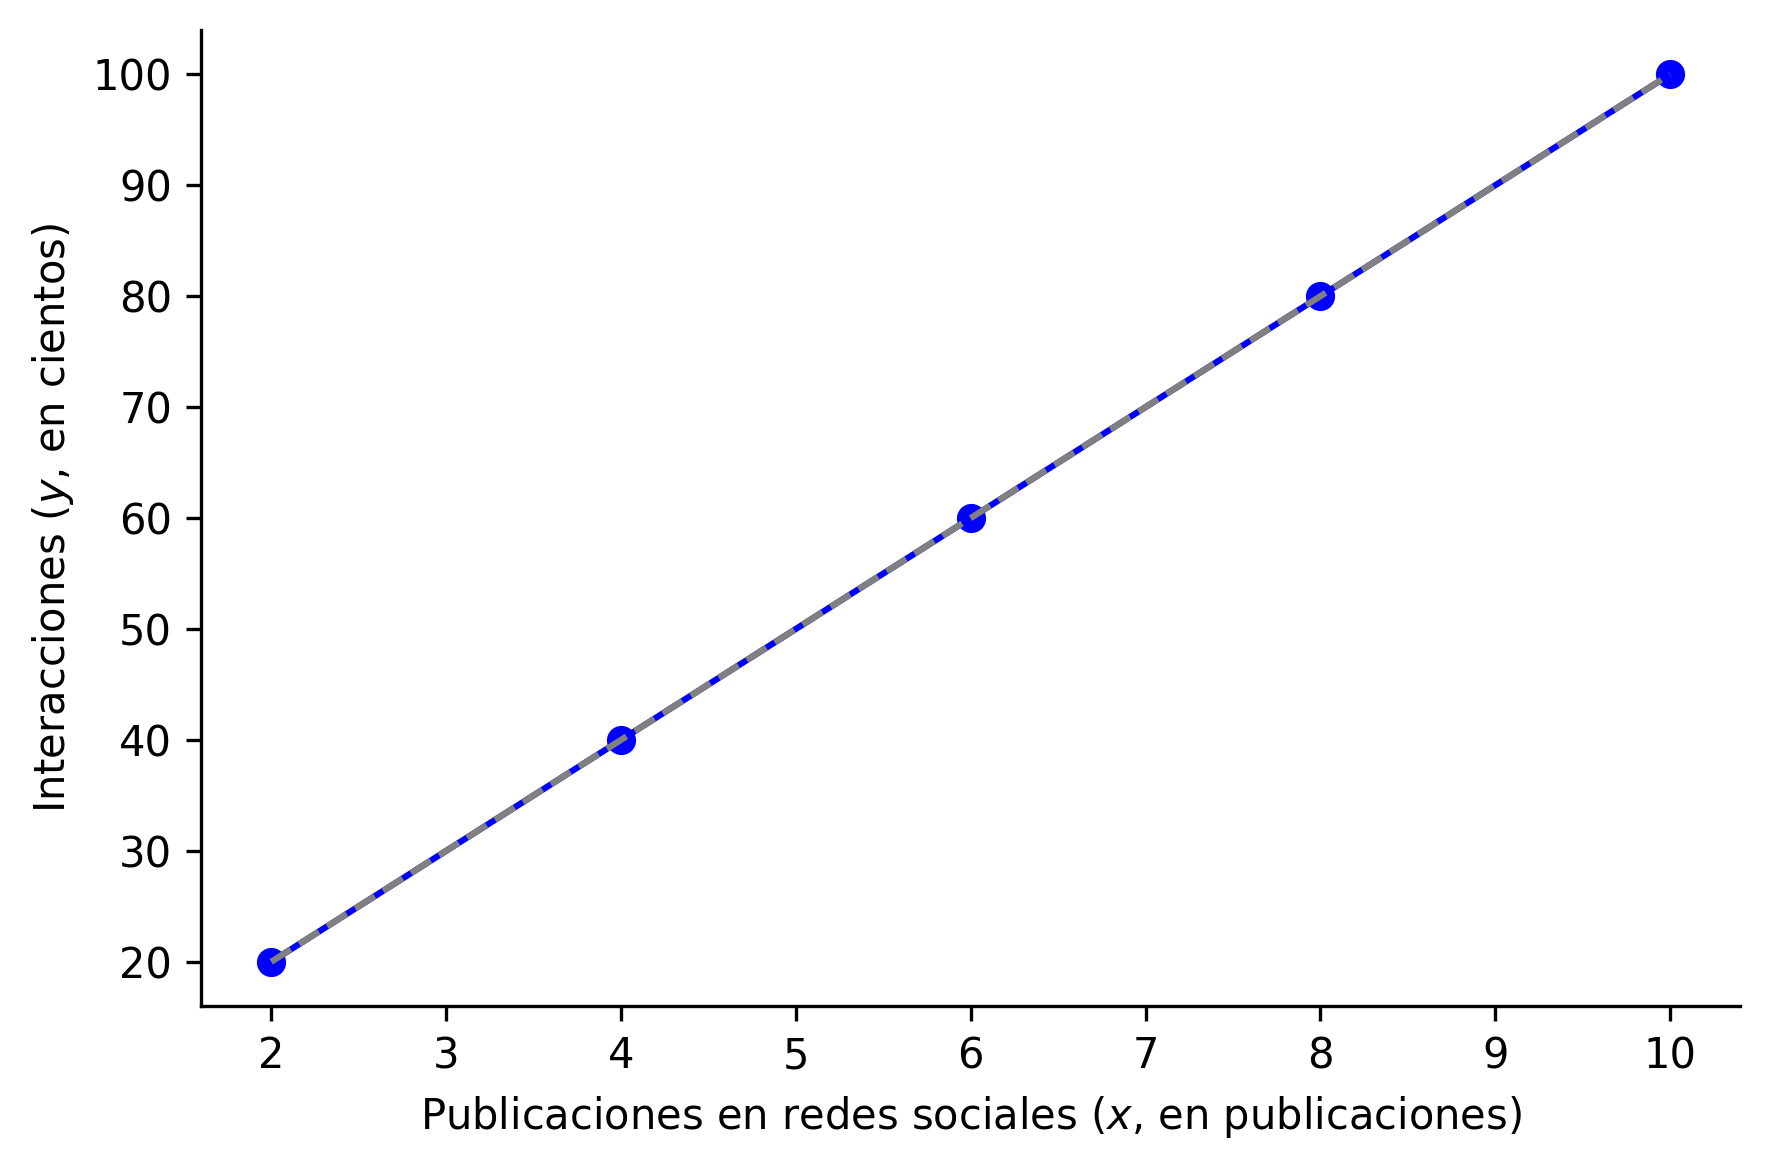
\includegraphics[keepaspectratio]{index_files/figure-pdf/cell-2-output-1.png}}

}

\end{figure}%

\subsection{Caso General}\label{caso-general}

Para cualquier par de magnitudes directamente proporcionales \(A\) e
\(B\), se cumple:

\begin{table}

{\caption{{Magnitudes directamente
proporcionales}{\label{tbl-mytable2}}}}

\begin{longtable}[]{@{}llll@{}}
\toprule\noalign{}
\(A\) & \(A_1\) & \(A_2\) & \(A_3\) \\
\midrule\noalign{}
\endhead
\bottomrule\noalign{}
\endlastfoot
\(B\) & \(B_1\) & \(B_2\) & \(B_3\) \\
\end{longtable}

{\noindent \emph{Note.} Elaboración propia}

\end{table}

La relación entre estas magnitudes satisface:

\[
\frac{A_1}{B_1} = \frac{A_2}{B_2} = \frac{A_3}{B_3} = k
\]

En general:

\[
\frac{A_i}{B_i} = k, \quad \text{donde } 1 \leq i < n, \quad i \in \mathbb{Z}
\]

Aquí, \(k\) es la \textbf{constante de proporcionalidad directa}.

\subsection{Función de Proporcionalidad
Directa}\label{funciuxf3n-de-proporcionalidad-directa}

La relación entre dos magnitudes directamente proporcionales se expresa
mediante una \textbf{función lineal homogénea}:

\[
f(x) = kx
\]

donde \(f(x)\) es la magnitud dependiente (en este caso, las
interacciones), \(x\) es la magnitud independiente (publicaciones) y
\(k\) es la constante de proporcionalidad.

\textbf{Ejemplo} Artículos Publicados y Lectores

Ahora, consideremos otro ejemplo. Supongamos que el \textbf{número de
artículos publicados} en un sitio web periodístico está relacionado con
el \textbf{número de lectores} que visitan el sitio:

\begin{table}

{\caption{{Relación entre Artículos publicados y
Lectores}{\label{tbl-mytable8}}}}

\begin{longtable}[]{@{}llllll@{}}
\toprule\noalign{}
Artículos publicados (\(x\)) & 1 & 2 & 3 & 4 & 5 \\
\midrule\noalign{}
\endhead
\bottomrule\noalign{}
\endlastfoot
Lectores (\(y\), en cientos) & 15 & 30 & 45 & 60 & 75 \\
\end{longtable}

{\noindent \emph{Note.} Elaboración propia}

\end{table}

La constante de proporcionalidad es:

\[
k = \frac{y}{x} = \frac{15}{1} = \frac{30}{2} = \frac{45}{3} = \frac{60}{4} = \frac{75}{5} = 15
\]

La función que describe esta relación es:

\[
y = 15x
\]

\subsection{Magnitudes Inversamente
Proporcionales}\label{magnitudes-inversamente-proporcionales}

Dos magnitudes son inversamente proporcionales si al aumentar una, la
otra disminuye en la misma proporción, y viceversa

Imagina un medio periodístico que verifica noticias antes de
publicarlas. A mayor \textbf{tiempo dedicado a verificar noticias},
menor es el \textbf{número de errores} en las publicaciones. La
siguiente tabla se muestra los datos:

\begin{table}

{\caption{{Relación entre Tiempo de verificación y Errores en
publicaciones}{\label{tbl-mytable10}}}}

\begin{longtable}[]{@{}
  >{\raggedright\arraybackslash}p{(\linewidth - 8\tabcolsep) * \real{0.7288}}
  >{\raggedright\arraybackslash}p{(\linewidth - 8\tabcolsep) * \real{0.0678}}
  >{\raggedright\arraybackslash}p{(\linewidth - 8\tabcolsep) * \real{0.0678}}
  >{\raggedright\arraybackslash}p{(\linewidth - 8\tabcolsep) * \real{0.0678}}
  >{\raggedright\arraybackslash}p{(\linewidth - 8\tabcolsep) * \real{0.0678}}@{}}
\toprule\noalign{}
\begin{minipage}[b]{\linewidth}\raggedright
Tiempo de verificación (\(x\), en horas)
\end{minipage} & \begin{minipage}[b]{\linewidth}\raggedright
1
\end{minipage} & \begin{minipage}[b]{\linewidth}\raggedright
2
\end{minipage} & \begin{minipage}[b]{\linewidth}\raggedright
4
\end{minipage} & \begin{minipage}[b]{\linewidth}\raggedright
8
\end{minipage} \\
\midrule\noalign{}
\endhead
\bottomrule\noalign{}
\endlastfoot
Errores en publicaciones (\(y\), en cantidad) & 40 & 20 & 10 & 5 \\
\end{longtable}

{\noindent \emph{Note.} Elaboración propia}

\end{table}

El tiempo de verificación y los errores en publicaciones son
\textbf{inversamente proporcionales}. Esto se verifica porque el
producto de ambas magnitudes es constante:

\[
(\text{Tiempo de verificación}) \cdot (\text{Errores}) = 1 \cdot 40 = 2 \cdot 20 = 4 \cdot 10 = 8 \cdot 5 = 40
\]

La \textbf{constante de proporcionalidad inversa} es:

\[
x \cdot y = 40
\]

La relación se expresa como:

\[
y = \frac{40}{x}
\]

\subsection{Representación
Gráfica}\label{representaciuxf3n-gruxe1fica-1}

La relación inversamente proporcional se visualiza como una curva
hiperbólica.

\begin{figure}[H]

\caption{Relación entre Tiempo de verificación y Errores en
publicaciones}

{\centering \pandocbounded{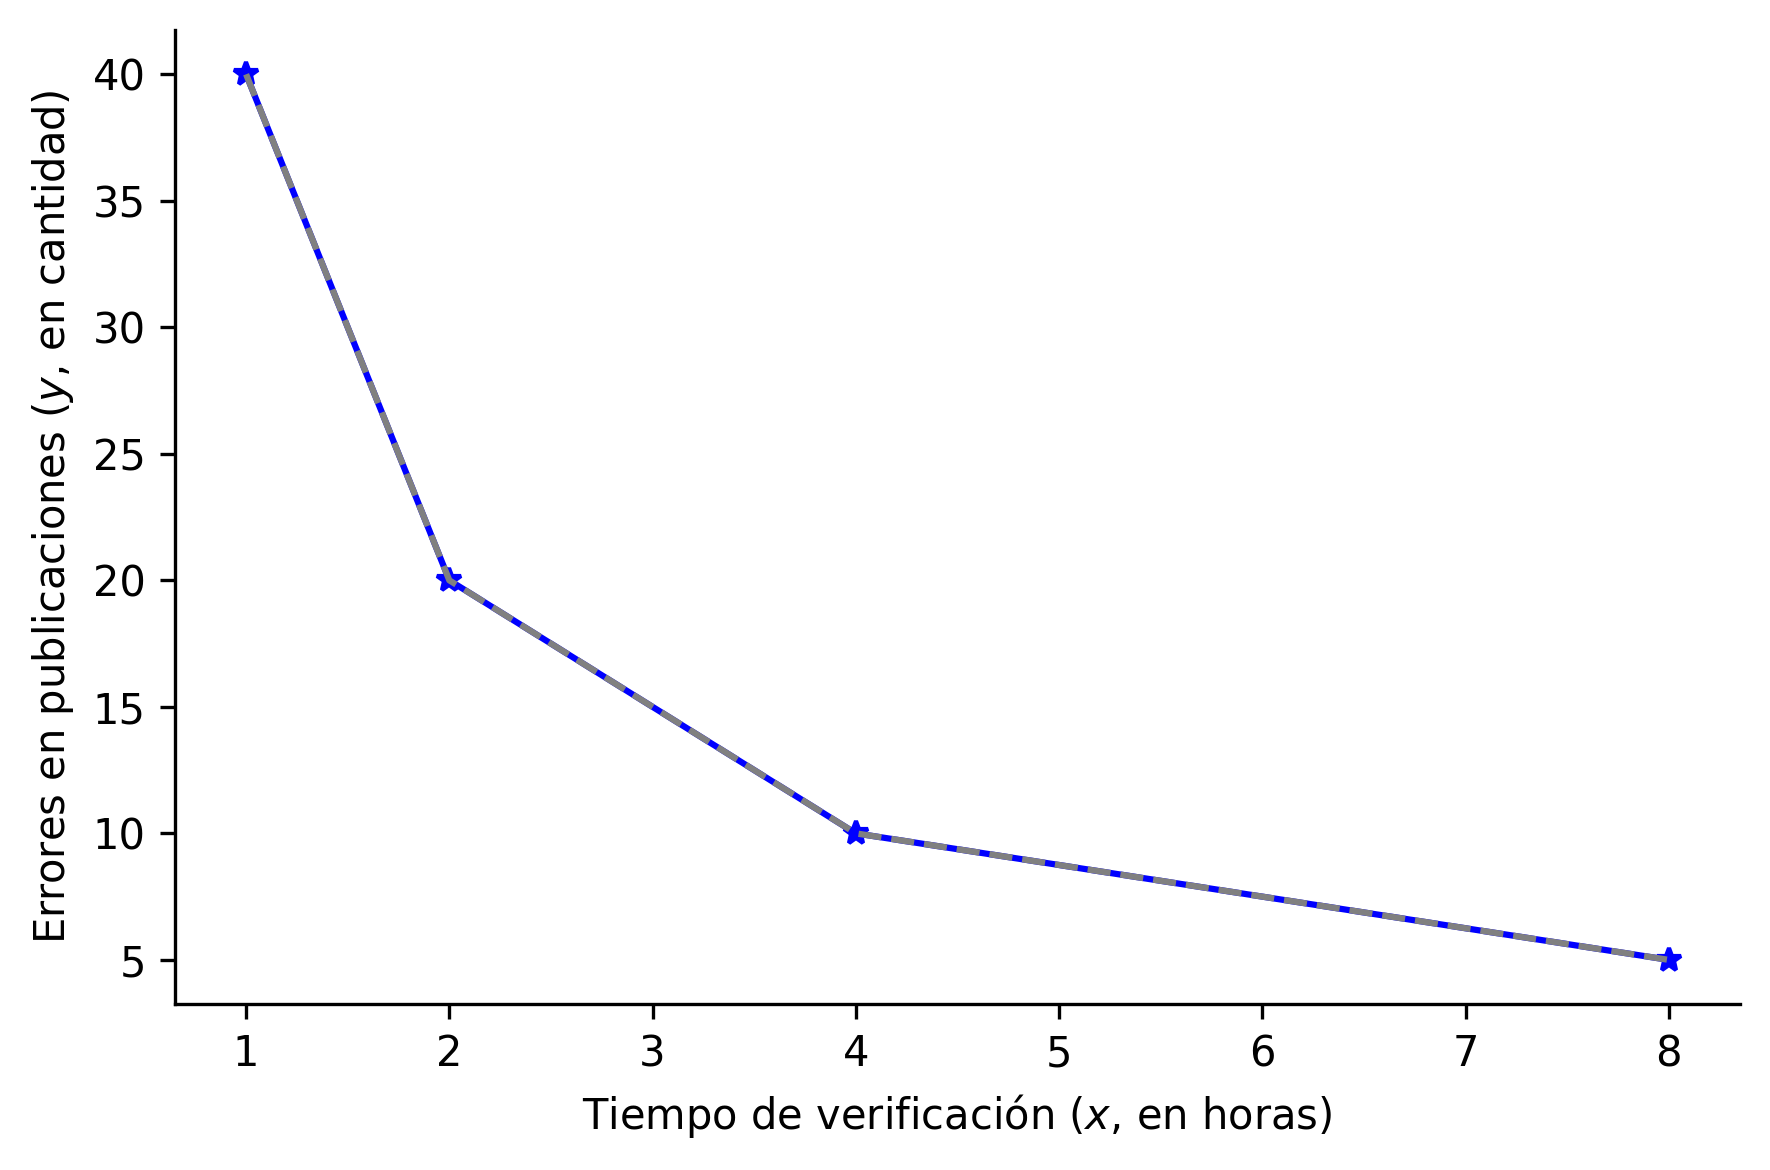
\includegraphics[keepaspectratio]{index_files/figure-pdf/cell-3-output-1.png}}

}

\end{figure}%

La gráfica muestra cómo, al aumentar el tiempo de verificación, el
número de errores disminuye, siguiendo una relación inversa.

\subsection{Caso General}\label{caso-general-1}

Para dos magnitudes inversamente proporcionales \(A\) e \(B\), se
cumple:

\begin{table}

{\caption{{Magnitudes inversamente
proporcionales}{\label{tbl-mytable11}}}}

\begin{longtable}[]{@{}llllll@{}}
\toprule\noalign{}
\(A\) & \(A_1\) & \(A_2\) & \(A_3\) & \(\dots\) & \(A_n\) \\
\midrule\noalign{}
\endhead
\bottomrule\noalign{}
\endlastfoot
\(B\) & \(B_1\) & \(B_2\) & \(B_3\) & \(\dots\) & \(B_n\) \\
\end{longtable}

{\noindent \emph{Note.} Elaboración propia}

\end{table}

El producto de las magnitudes es constante:

\[
A_1 \cdot B_1 = A_2 \cdot B_2 = A_3 \cdot B_3 = \dots = A_n \cdot B_n = k
\]

En general:

\[
A_i \cdot B_i = k, \quad \text{donde } 1 \leq i < n, \quad i \in \mathbb{Z}
\]

Aquí, \(k\) es la \textbf{constante de proporcionalidad inversa}.

\subsection{Función de Proporcionalidad
Inversa}\label{funciuxf3n-de-proporcionalidad-inversa}

La relación inversamente proporcional se expresa como:

\[
y = \frac{k}{x}
\]

donde \(y\) es la magnitud dependiente (errores), \(x\) es la magnitud
independiente (tiempo de verificación) y \(k\) es la constante de
proporcionalidad inversa.

\textbf{Ejemplo} Frecuencia de Titulares Clickbait y Confianza del
Lector

Consideremos otro ejemplo: la relación entre la \textbf{frecuencia de
titulares clickbait} (titulares exagerados para atraer clics) y la
\textbf{confianza del lector} en un medio:

\begin{table}

{\caption{{Relación entre Frecuencia de titulares clickbait y Confianza
del lector}{\label{tbl-mytable12}}}}

\begin{longtable}[]{@{}
  >{\raggedright\arraybackslash}p{(\linewidth - 8\tabcolsep) * \real{0.7612}}
  >{\raggedright\arraybackslash}p{(\linewidth - 8\tabcolsep) * \real{0.0597}}
  >{\raggedright\arraybackslash}p{(\linewidth - 8\tabcolsep) * \real{0.0597}}
  >{\raggedright\arraybackslash}p{(\linewidth - 8\tabcolsep) * \real{0.0597}}
  >{\raggedright\arraybackslash}p{(\linewidth - 8\tabcolsep) * \real{0.0597}}@{}}
\toprule\noalign{}
\begin{minipage}[b]{\linewidth}\raggedright
Frecuencia de titulares clickbait (\(x\), por semana)
\end{minipage} & \begin{minipage}[b]{\linewidth}\raggedright
12
\end{minipage} & \begin{minipage}[b]{\linewidth}\raggedright
4
\end{minipage} & \begin{minipage}[b]{\linewidth}\raggedright
2.4
\end{minipage} & \begin{minipage}[b]{\linewidth}\raggedright
1.3
\end{minipage} \\
\midrule\noalign{}
\endhead
\bottomrule\noalign{}
\endlastfoot
Confianza del lector (\(y\), en escala 1-50) & 5 & 15 & 25 & 45 \\
\end{longtable}

{\noindent \emph{Note.} Elaboración propia}

\end{table}

El producto es constante:

\[
12 \cdot 5 = 4 \cdot 15 = 2.4 \cdot 25 = 1.3 \cdot 45 = 60
\]

La constante de proporcionalidad inversa es:

\[
x \cdot y = 60
\]

La función es:

\[
y = \frac{60}{x}
\]

\subsection{Propiedades}\label{propiedades}

Sean las magnitudes \(A\) y \(B\), entonces:

\begin{enumerate}
\def\labelenumi{\arabic{enumi}.}
\tightlist
\item
  Si \(A \text{ DP } B \Rightarrow B \text{ DP } A\)
\item
  Si \(A \text{ IP } B \Rightarrow B \text{ IP } A\)
\item
  \(A \text{ IP } B \Leftrightarrow A \text{ DP } \left( \frac{1}{B} \right)\)
\item
  \(A \text{ DP } B \Leftrightarrow A \text{ IP } \left( \frac{1}{B} \right)\)
\item
  Si \(n \in \mathbb{Q}\), entonces:

  \begin{itemize}
  \tightlist
  \item
    \(A \text{ DP } B \Leftrightarrow A^n \text{ DP } B^n\)
  \item
    \(A \text{ IP } B \Leftrightarrow A^n \text{ IP } B^n\)
  \end{itemize}
\end{enumerate}

\section{Aplicaciones de las Magnitudes
Proporcionales}\label{aplicaciones-de-las-magnitudes-proporcionales}

Las magnitudes proporcionales permiten distribuir cantidades de forma
equitativa según una relación directa o inversa. Este proceso, conocido
como \textbf{reparto proporcional}, asigna una cantidad total entre
varias partes según una variable de referencia. Se divide en dos tipos:
\textbf{reparto directo} y \textbf{reparto inverso}.

\subsection{Reparto Directo}\label{reparto-directo}

El reparto directo distribuye una cantidad total entre varias partes
proporcionalmente a sus magnitudes. Por ejemplo, supongamos que se desea
repartir un presupuesto de S/ 12,000 entre tres proyectos según el
número de publicaciones planificadas, con proporciones de 1, 3 y 4.

Calculamos:

\[
\text{Total a repartir: } 12,000
\]

\begin{align*}
\begin{cases}
1k = \text{Monto para el primer proyecto} \\
3k = \text{Monto para el segundo proyecto} \\
4k = \text{Monto para el tercer proyecto} \\
\end{cases}
\end{align*}

La suma total es:

\[
1k + 3k + 4k = 8k = 12,000
\]

Resolviendo para \(k\):

\[
k = \frac{12,000}{8} = 1,500
\]

Por lo tanto, los montos asignados son:

\begin{align*}
\begin{cases}
1k = 1 \cdot 1,500 = 1,500 \\
3k = 3 \cdot 1,500 = 4,500 \\
4k = 4 \cdot 1,500 = 6,000 \\
\end{cases}
\end{align*}

Los proyectos reciben S/ 1,500, S/ 4,500 y S/ 6,000, respectivamente.

\subsubsection{Gráfica del Reparto
Directo}\label{gruxe1fica-del-reparto-directo}

La siguiente gráfica ilustra cómo se distribuye el presupuesto según las
proporciones:

\begin{figure}[H]

\caption{Distribución del presupuesto según número de publicaciones}

{\centering \pandocbounded{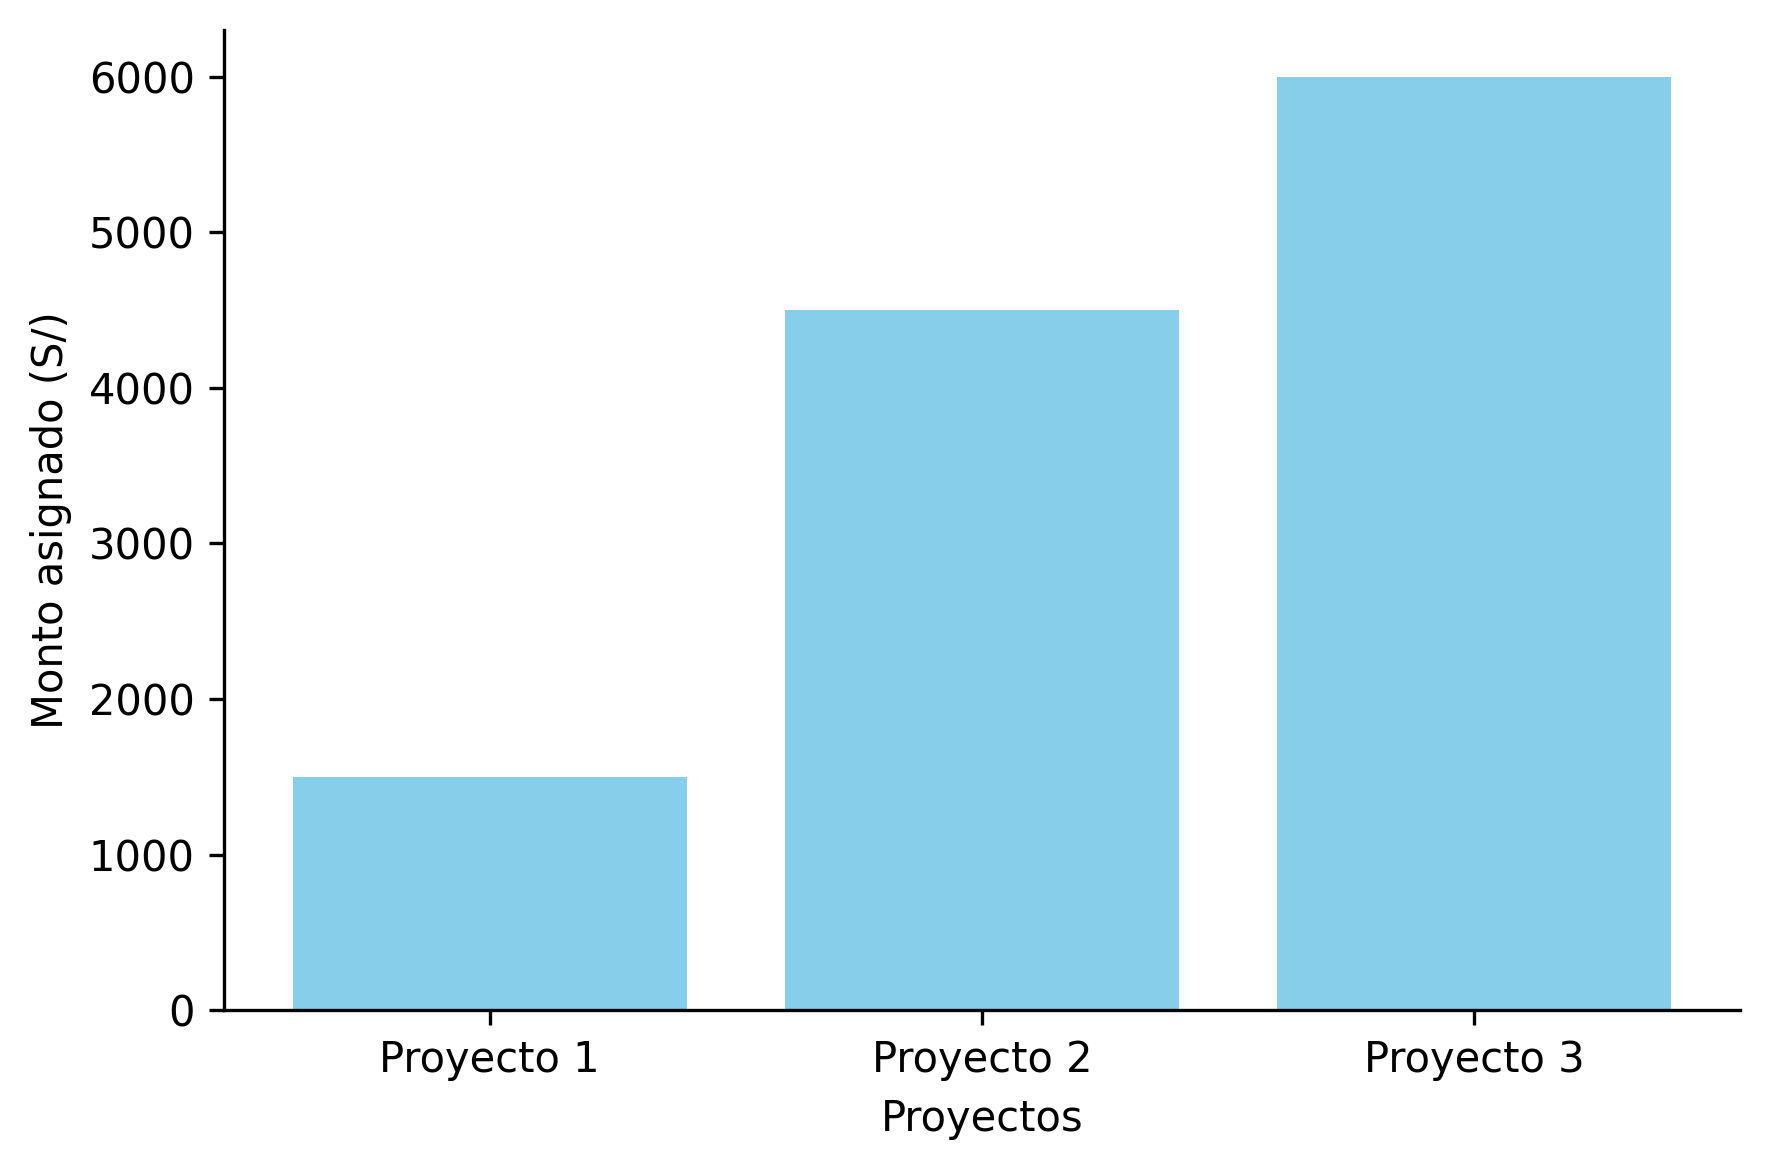
\includegraphics[keepaspectratio]{index_files/figure-pdf/cell-4-output-1.png}}

}

\end{figure}%

\subsection{Reparto Inverso}\label{reparto-inverso}

El reparto inverso distribuye una cantidad total entre varias partes de
forma inversamente proporcional a sus magnitudes. Por ejemplo,
supongamos que se desea repartir un fondo de S/ 60,000 entre tres
equipos según el tiempo de entrega de artículos, con proporciones de 1,
2 y 4 horas.

La distribución se calcula como sigue:

\[
\text{Total a repartir: } 60,000
\]

\begin{align*}
\begin{cases}
\frac{k}{1} = \text{Monto para el primer equipo} \\
\frac{k}{2} = \text{Monto para el segundo equipo} \\
\frac{k}{4} = \text{Monto para el tercer equipo} \\
\end{cases}
\end{align*}

La suma total es:

\[
\frac{k}{1} + \frac{k}{2} + \frac{k}{4} = k \left(1 + \frac{1}{2} + \frac{1}{4}\right) = k \cdot \frac{7}{4} = 60,000
\]

Resolviendo para \(k\):

\[
k = \frac{60,000 \cdot 4}{7} \approx 34,285.71
\]

Por lo tanto, los montos asignados son:

\begin{align*}
\begin{cases}
\frac{k}{1} \approx \frac{34,285.71}{1} \approx 34,285.71 \\
\frac{k}{2} \approx \frac{34,285.71}{2} \approx 17,142.86 \\
\frac{k}{4} \approx \frac{34,285.71}{4} \approx 8,571.43 \\
\end{cases}
\end{align*}

Los equipos reciben aproximadamente S/ 34,286, S/ 17,143 y S/ 8,571,
respectivamente.

\subsubsection{Gráfica del Reparto
Inverso}\label{gruxe1fica-del-reparto-inverso}

La siguiente gráfica se muestra cómo se distribuye el fondo según el
tiempo de entrega:

\begin{figure}[H]

\caption{Distribución del fondo según tiempo de entrega}

{\centering \pandocbounded{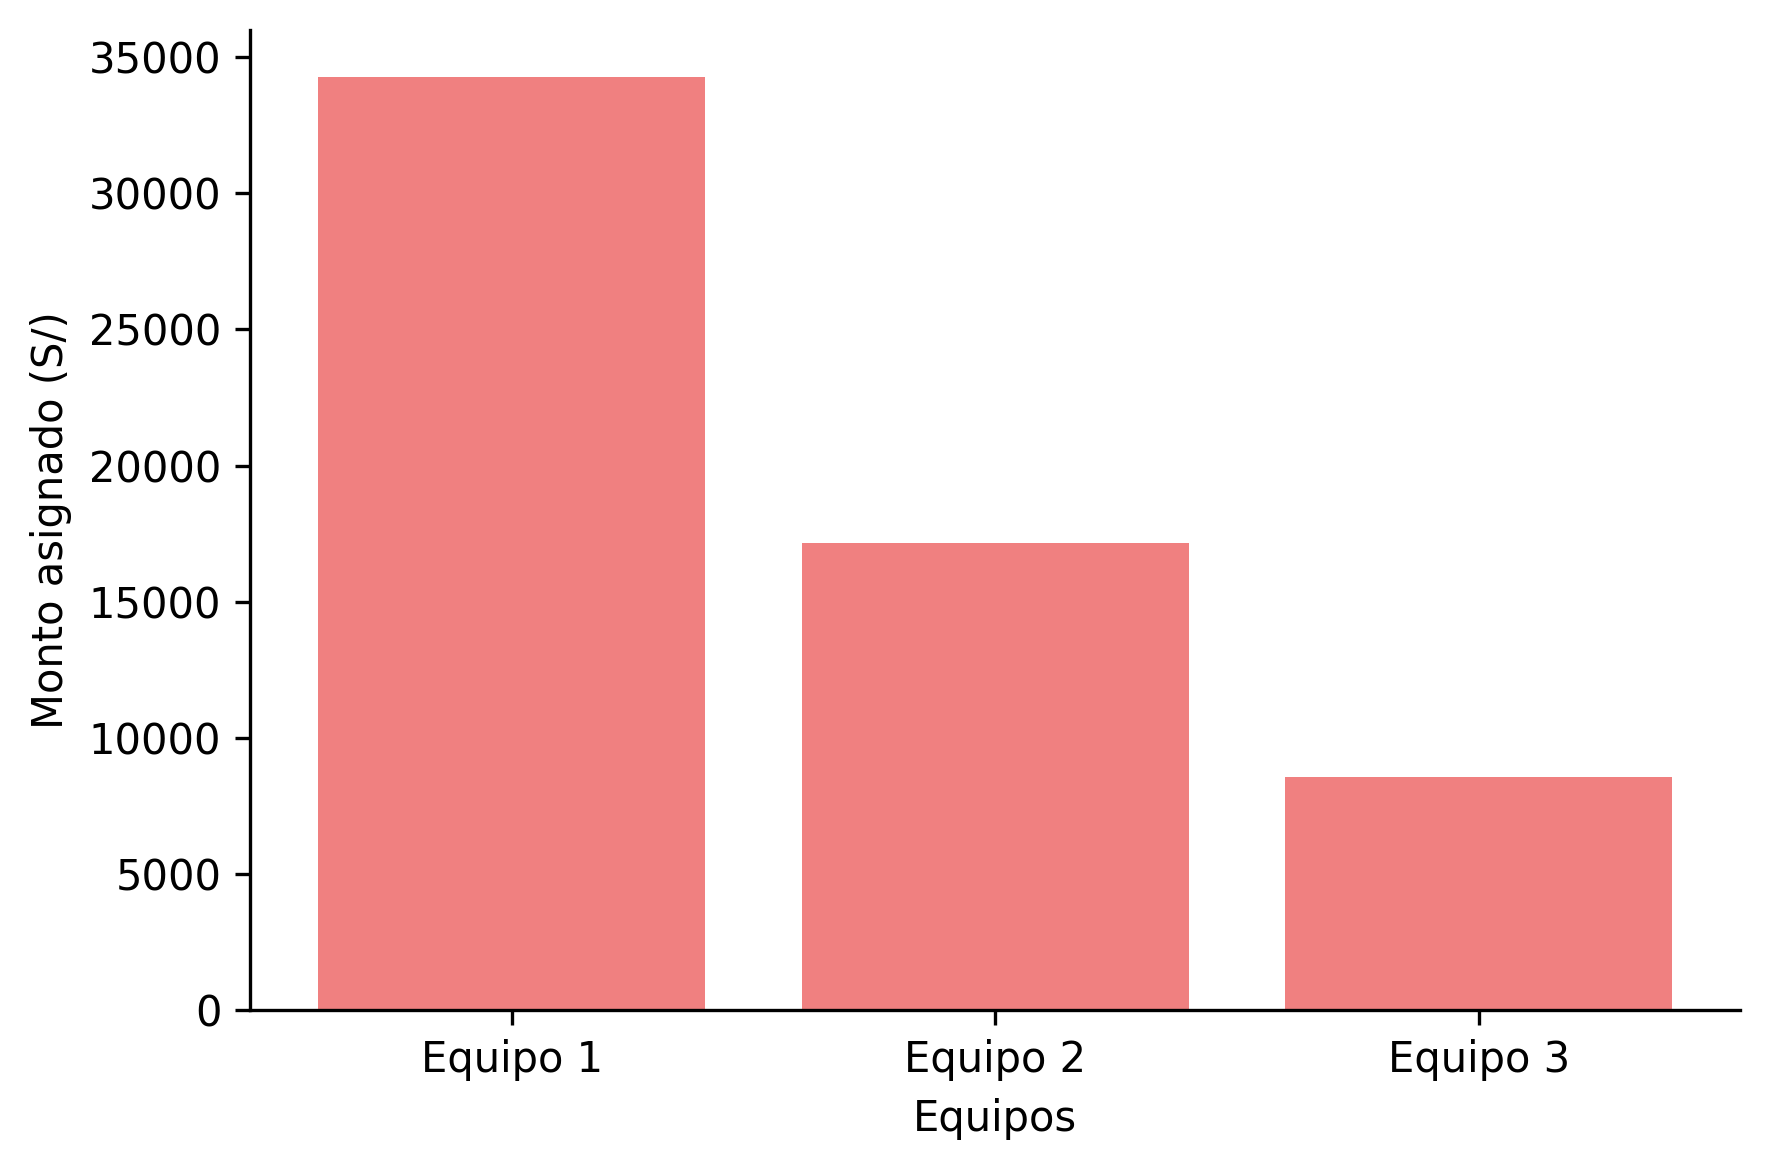
\includegraphics[keepaspectratio]{index_files/figure-pdf/cell-5-output-1.png}}

}

\end{figure}%

\section{Regla de Tres y Porcentajes}\label{regla-de-tres-y-porcentajes}

La regla de tres y los porcentajes son herramientas matemáticas
esenciales para resolver problemas de proporcionalidad y comparación de
datos.

\subsection{Regla de Tres}\label{regla-de-tres}

La \textbf{regla de tres} permite encontrar un valor desconocido a
partir de tres valores conocidos, en relaciones de proporcionalidad
directa o inversa.

\subsubsection{Regla de Tres Simple
Directa}\label{regla-de-tres-simple-directa}

En una relación \textbf{directamente proporcional}, si una magnitud
aumenta, la otra también lo hace en la misma proporción, cumpliendo:

\[
\frac{\text{Magnitud 1}}{\text{Magnitud 2}} = k
\]

De forma práctica, se multiplica en cruz:

\[
a \cdot x = b \cdot c \quad \Rightarrow \quad x = \frac{b \cdot c}{a}
\]

\textbf{Ejemplo}: Si escribir 2 artículos toma 4 horas, ¿cuánto tiempo
tomará escribir 5 artículos?

Planteamos:

\[
\frac{2 \text{ artículos}}{4 \text{ horas}} = \frac{5 \text{ artículos}}{x \text{ horas}}
\]

Multiplicamos en cruz:

\[
2 \cdot x = 4 \cdot 5 \quad \Rightarrow \quad 2x = 20 \quad \Rightarrow \quad x = \frac{20}{2} = 10
\]

Tomará 10 horas escribir 5 artículos.

\paragraph{Gráfica de la Regla de Tres
Directa.}\label{gruxe1fica-de-la-regla-de-tres-directa}

La siguiente gráfica muestra la relación proporcional entre artículos y
tiempo:

\begin{figure}[H]

\caption{Relación entre número de artículos y tiempo de escritura}

{\centering \pandocbounded{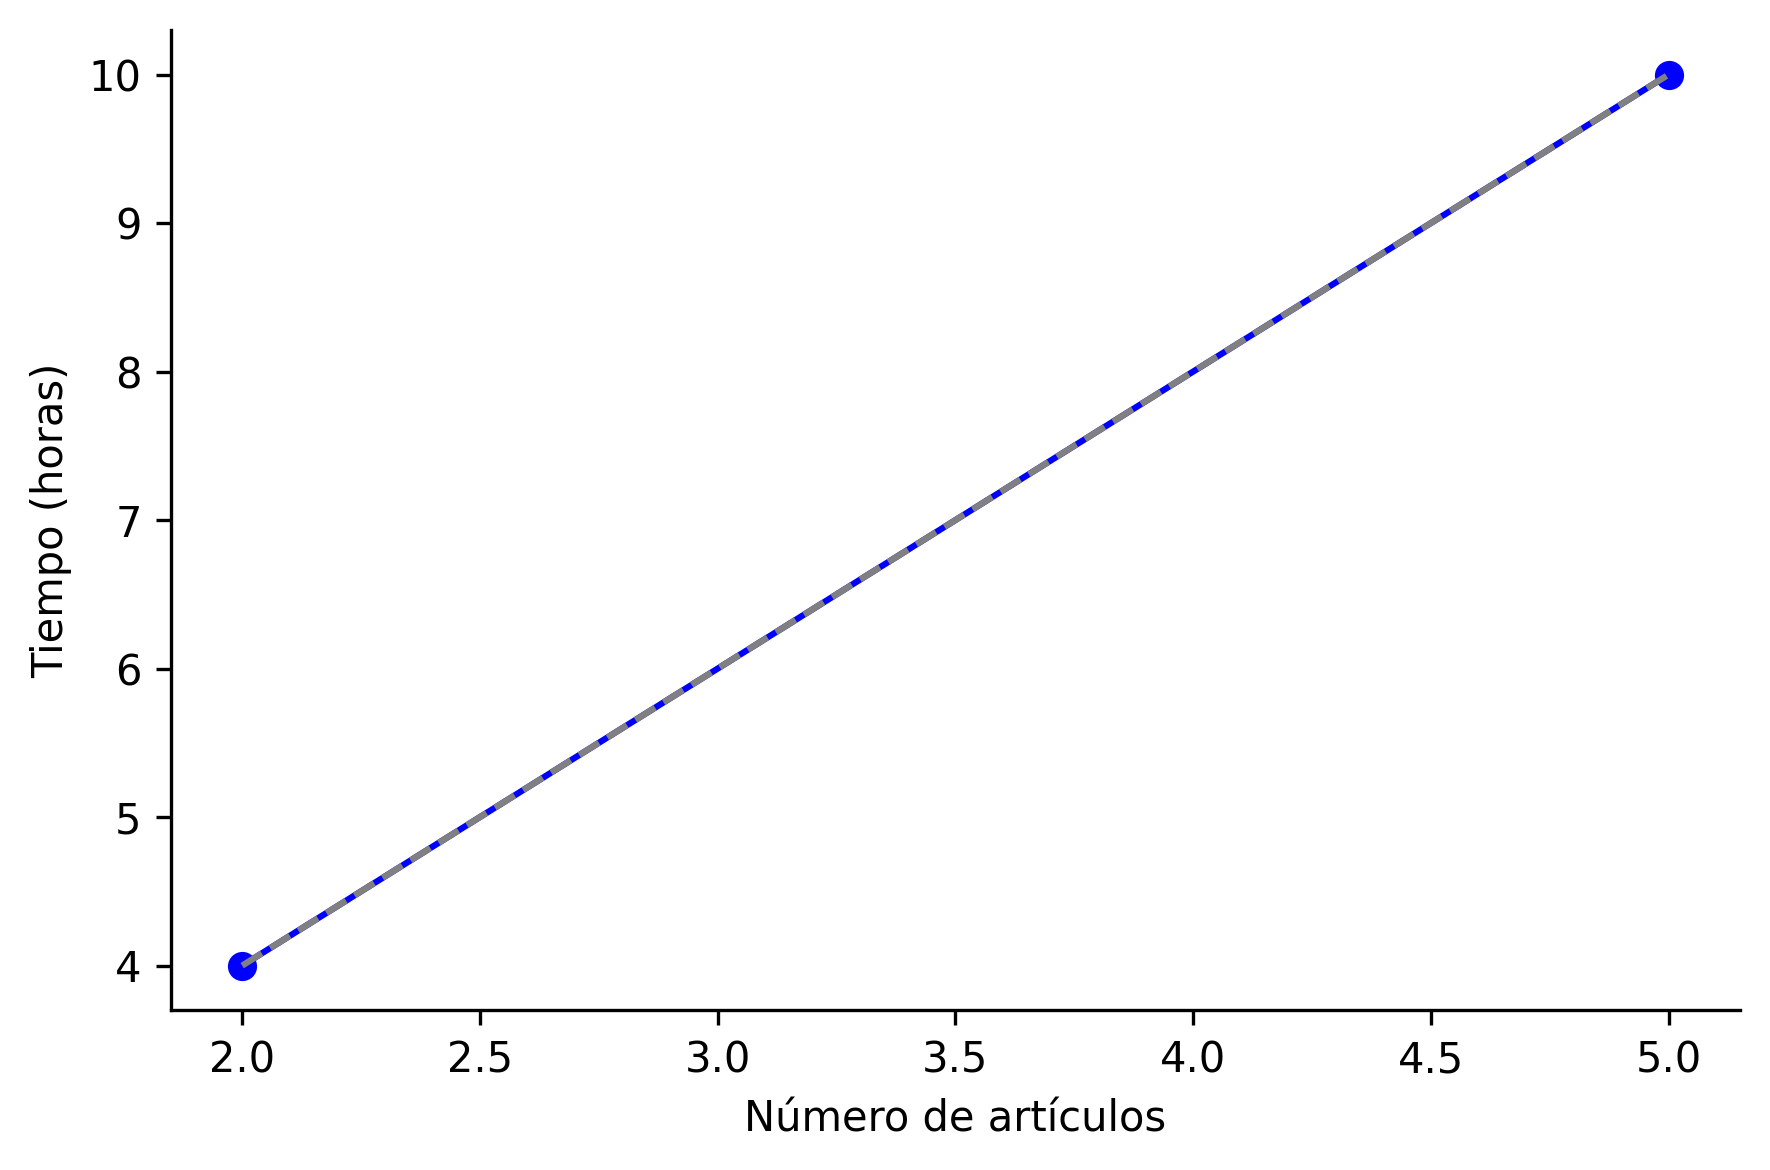
\includegraphics[keepaspectratio]{index_files/figure-pdf/cell-6-output-1.png}}

}

\end{figure}%

\subsubsection{Regla de Tres Simple
Inversa}\label{regla-de-tres-simple-inversa}

En una relación \textbf{inversamente proporcional}, si una magnitud
aumenta, la otra disminuye, cumpliendo:

\[
\text{Magnitud 1} \cdot \text{Magnitud 2} = k
\]

De forma práctica, se multiplica en paralelo:

\[
a \cdot b = c \cdot x \quad \Rightarrow \quad x = \frac{a \cdot b}{c}
\]

\textbf{Ejemplo}: Si con 4 máquinas se imprimen 200 revistas en 8 horas,
¿cuánto tiempo tomará con 12 máquinas?

Planteamos:

\[
4 \cdot 8 = 12 \cdot x
\]

Resolviendo:

\[
4 \cdot 8 = 12x \quad \Rightarrow \quad 32 = 12x \quad \Rightarrow \quad x = \frac{32}{12} \approx 2.67
\]

Con 12 máquinas, tomará aproximadamente 2.67 horas.

\paragraph{Gráfica de la Regla de Tres
Inversa.}\label{gruxe1fica-de-la-regla-de-tres-inversa}

La siguiente gráfica muestra la relación inversa entre máquinas y
tiempo:

\begin{figure}[H]

\caption{Relación entre número de máquinas y tiempo de impresión}

{\centering \pandocbounded{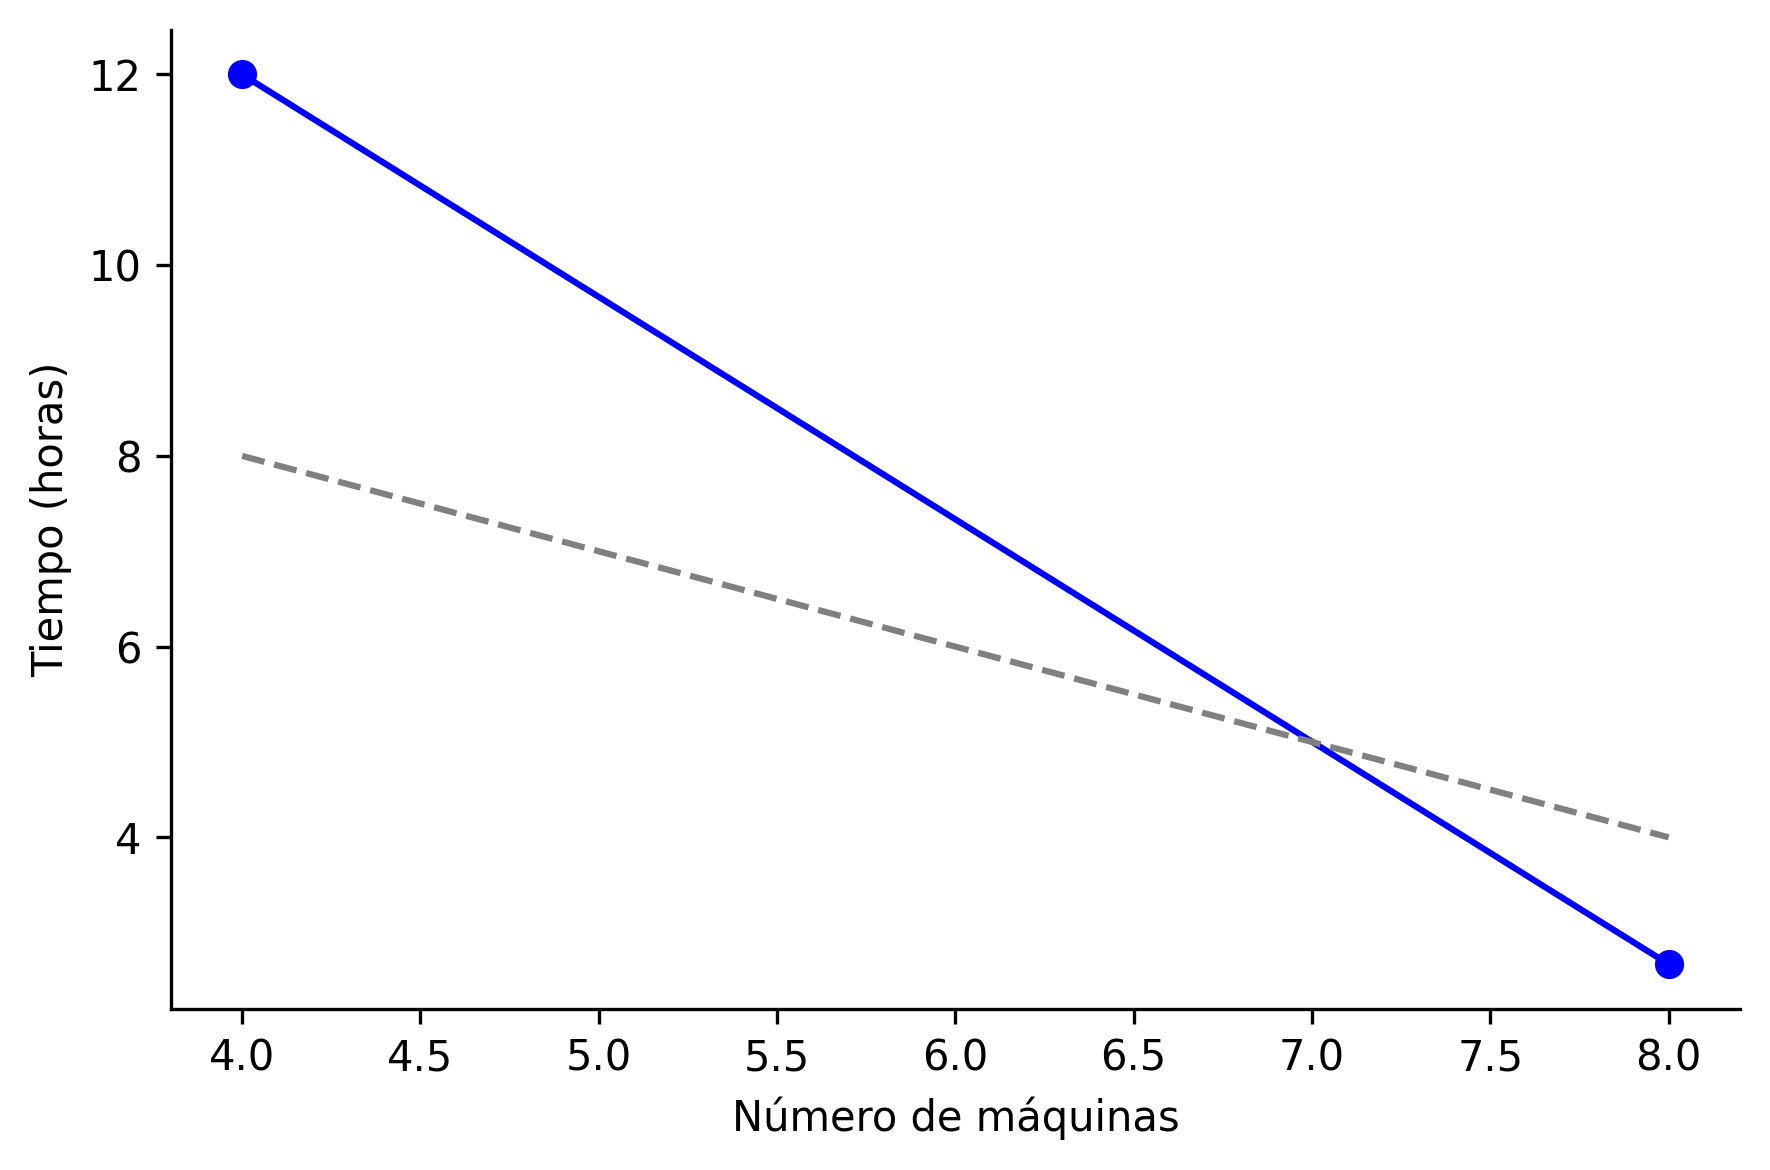
\includegraphics[keepaspectratio]{index_files/figure-pdf/cell-7-output-1.png}}

}

\end{figure}%

\subsubsection{Regla de Tres Compuesta}\label{regla-de-tres-compuesta}

La \textbf{regla de tres compuesta} se usa cuando más de dos magnitudes
están involucradas. Se combinan proporciones directas e inversas para
resolver el problema.

\textbf{Ejemplo}: Si 3 periodistas escriben 6 artículos en 12 horas,
¿cuánto tiempo tomará a 6 periodistas escribir 12 artículos?

\begin{itemize}
\tightlist
\item
  \textbf{Proporción directa} (artículos): Más artículos requieren más
  tiempo.
\item
  \textbf{Proporción inversa} (journalistas): Más periodistas reducen el
  tiempo.
\end{itemize}

Planteamos:

\[
\frac{3 \text{ periodistas} \cdot 12 \text{ horas}}{6 \text{ artículos}} = \frac{6 \text{ periodistas} \cdot x \text{ horas}}{12 \text{ artículos}}
\]

Simplificando:

\[
\frac{3 \cdot 12}{6} = \frac{6 \cdot x}{12}
\]

\[
\frac{36}{6} = \frac{6x}{12} \quad \Rightarrow \quad 6 = \frac{6x}{12} \quad \Rightarrow \quad 6 \cdot 12 = 6x \quad \Rightarrow \quad 72 = 6x \quad \Rightarrow \quad x = 12
\]

Tomará 12 horas.

\subsection{Porcentajes}\label{porcentajes}

El \textbf{porcentaje} expresa una proporción en términos de ``por cada
cien'', facilitando la comparación de datos. La fórmula para calcular un
porcentaje es:

\[
\text{a por ciento de N} = a% \text{ de } N = \frac{a}{100} \cdot N
\]

\textbf{Ejemplo}: Calcular el 25\% de 200 lectores.

\[
25% \text{ de } 200 = \frac{25}{100} \cdot 200 = 50
\]

50 lectores representan el 25\% de 200.

\subsubsection{Parte de un Total como
Porcentaje}\label{parte-de-un-total-como-porcentaje}

Para expresar una parte de un total en porcentaje:

\[
\frac{\text{Parte}}{\text{Total}} \cdot 100% = \frac{a}{b} \cdot 100%
\]

\textbf{Ejemplo}: Si 30 de 150 suscriptores leen un artículo, ¿qué
porcentaje representa?

\[
\frac{30}{150} \cdot 100% = 20%
\]

El 20\% de los suscriptores leyeron el artículo.

\subsubsection{Operaciones con
Porcentajes}\label{operaciones-con-porcentajes}

Un número se puede expresar como el 100\% de sí mismo:

\[
N = 100% \cdot N
\]

\textbf{Ejemplo}: Si el 40\% de un presupuesto más el 60\% del mismo
presupuesto se usan, ¿qué porcentaje total se gastó?

\[
40%N + 60%N = 100%N
\]

Se gastó el 100\% del presupuesto.

\subsubsection{Aplicaciones de los
Porcentajes}\label{aplicaciones-de-los-porcentajes}

\paragraph{a. Descuentos Sucesivos.}\label{a.-descuentos-sucesivos}

Para dos descuentos consecutivos de \(a%
\) y \(b%
\), el descuento único equivalente es:

\[
\text{Descuento único} = (a + b) - \frac{a \cdot b}{100}
\]

\textbf{Ejemplo}: Un equipo de publicidad aplica descuentos del 10\% y
20\% en un contrato. ¿Cuál es el descuento único equivalente?

\[
\text{Descuento único} = (10 + 20) - \frac{10 \cdot 20}{100} = 30 - 2 = 28
\]

El descuento único es del 28\%.

\paragraph{b. Aumentos Sucesivos.}\label{b.-aumentos-sucesivos}

Para dos incrementos consecutivos de \(a%
\) y \(b%
\), el aumento único equivalente es:

\[
\text{Aumento único} = (a + b) + \frac{a \cdot b}{100}
\]

\textbf{Ejemplo}: Si un presupuesto aumenta un 15\% y luego un 10\%,
¿cuál es el aumento único equivalente?

\[
\text{Aumento único} = (15 + 10) + \frac{15 \cdot 10}{100} = 25 + 1.5 = 26.5
\]

El aumento único es del 26.5\%.

\section{Ejemplos Aplicados a Ciencias de la
Comunicación}\label{ejemplos-aplicados-a-ciencias-de-la-comunicaciuxf3n}

\subsection{Ejercicio 1}\label{ejercicio-1}

\textbf{Problema}: Si producir 3 videos promocionales requiere 9 horas
de trabajo, ¿cuánto tiempo tomará producir 7 videos?

\textbf{Solución}:

Dado que el número de videos y el tiempo de trabajo son directamente
proporcionales, usamos la regla de tres simple directa:

\[
\frac{\text{Magnitud 1}}{\text{Magnitud 2}} = k \quad \Rightarrow \quad a \cdot x = b \cdot c \quad \Rightarrow \quad x = \frac{b \cdot c}{a}
\]

Planteamos la proporción:

\[
\frac{3 \text{ videos}}{9 \text{ horas}} = \frac{7 \text{ videos}}{x \text{ horas}}
\]

Multiplicamos en cruz:

\[
3 \cdot x = 9 \cdot 7
\]

\[
3x = 63 \quad \Rightarrow \quad x = \frac{63}{3} = 21
\]

Se necesitan 21 horas para producir 7 videos.

\textbf{Gráfica}:

\begin{figure}[H]

\caption{Relación entre número de videos y tiempo de producción}

{\centering \pandocbounded{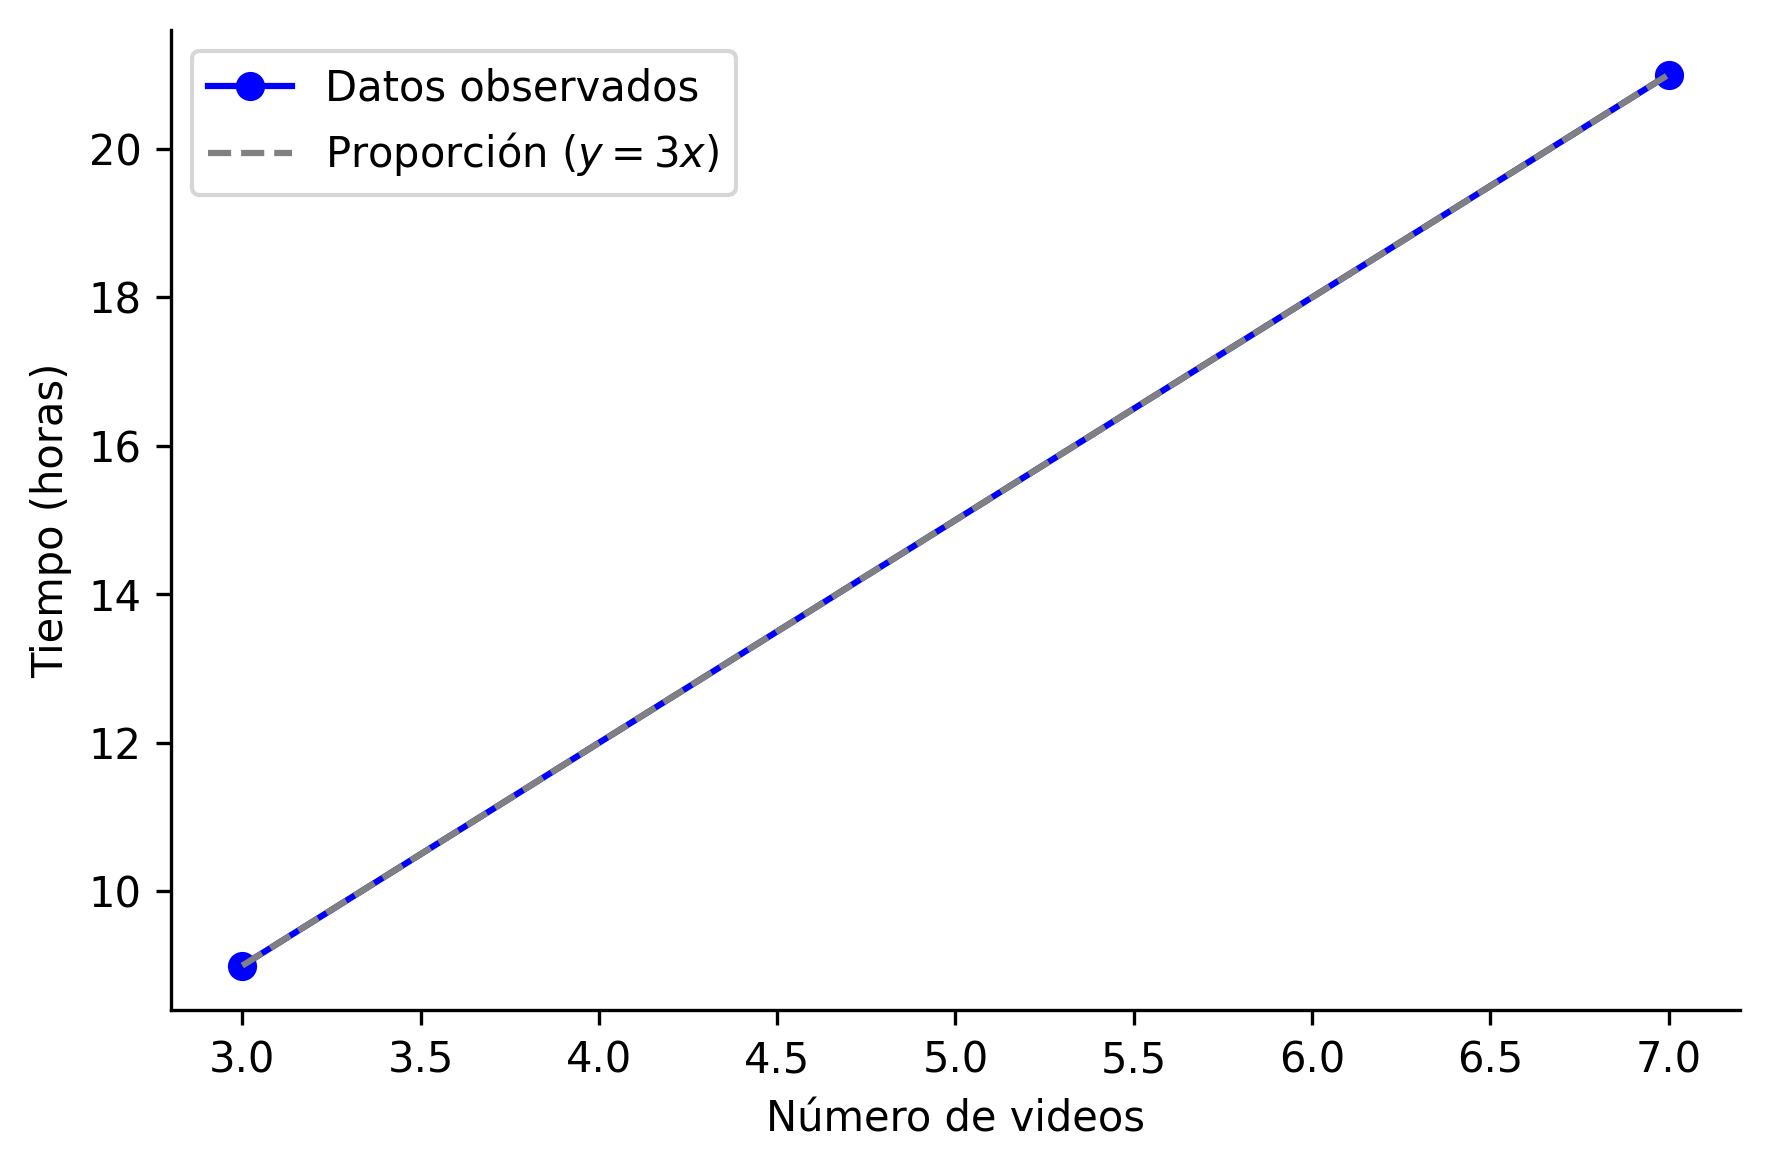
\includegraphics[keepaspectratio]{index_files/figure-pdf/cell-8-output-1.png}}

}

\end{figure}%

\subsection{Ejercicio 2}\label{ejercicio-2}

\textbf{Problema}: Si 5 diseñadores tardan 10 días en crear 100
gráficos, ¿cuántos días tardarán 10 diseñadores en crear los mismos 100
gráficos?

\textbf{Solución}:

Dado que el número de diseñadores y el tiempo son inversamente
proporcionales (a más diseñadores, menos tiempo), usamos la regla de
tres simple inversa:

\[
\text{Magnitud 1} \cdot \text{Magnitud 2} = k \quad \Rightarrow \quad a \cdot b = c \cdot x \quad \Rightarrow \quad x = \frac{a \cdot b}{c}
\]

Planteamos:

\[
5 \text{ diseñadores} \cdot 10 \text{ días} = 10 \text{ diseñadores} \cdot x \text{ días}
\]

Multiplicamos en paralelo:

\[
5 \cdot 10 = 10 \cdot x
\]

\[
50 = 10x \quad \Rightarrow \quad x = \frac{50}{10} = 5
\]

Con 10 diseñadores, se tardarán 5 días.

\textbf{Gráfica}:

\begin{figure}[H]

\caption{Relación entre número de diseñadores y tiempo de creación}

{\centering \pandocbounded{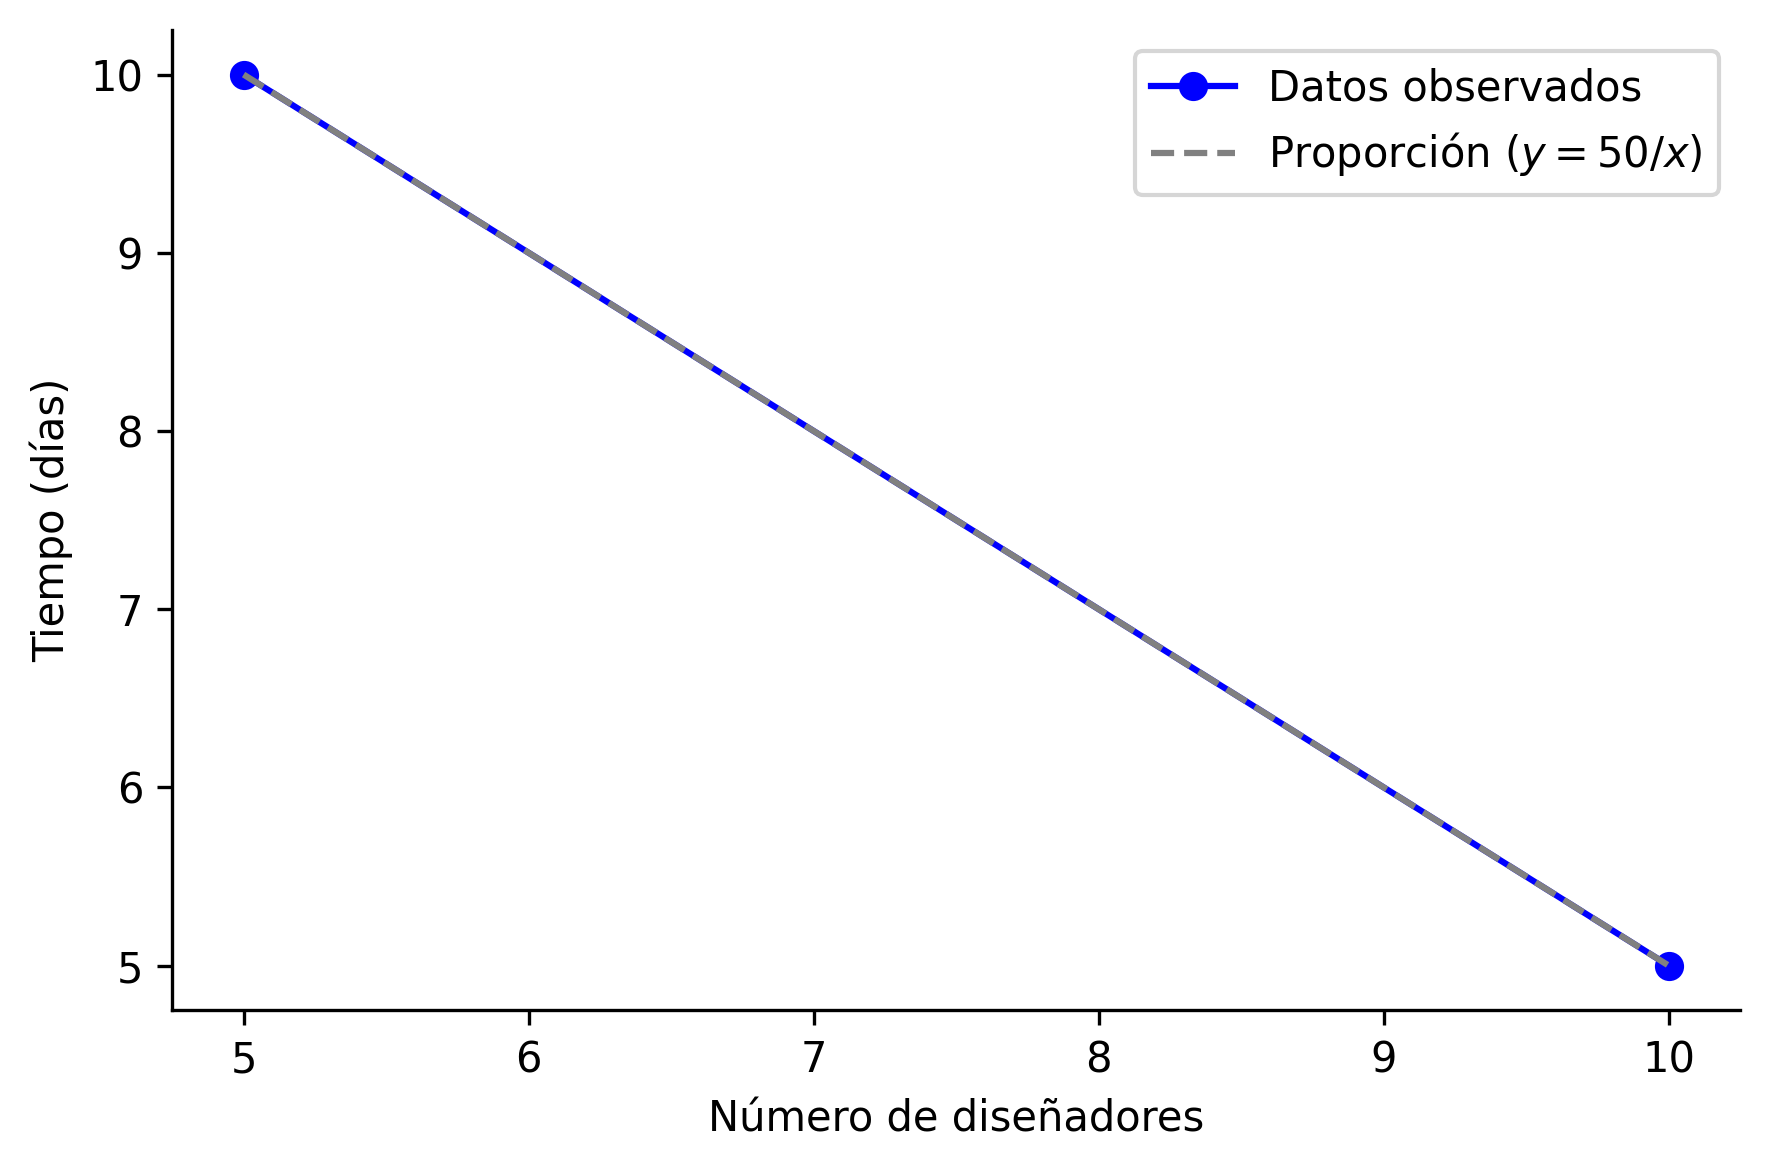
\includegraphics[keepaspectratio]{index_files/figure-pdf/cell-9-output-1.png}}

}

\end{figure}%

\subsection{Ejercicio 3}\label{ejercicio-3}

\textbf{Problema}: Se desea repartir un presupuesto de S/ 15,000 entre
tres campañas según el número de anuncios planificados, con proporciones
de 2, 3 y 5. ¿Cuánto recibirá cada campaña?

\textbf{Solución}:

Usamos el reparto proporcional directo, donde el presupuesto se
distribuye según las proporciones:

\[
\text{Total a repartir: } 15,000
\]

Asignamos:

\[
\begin{cases}
2k = \text{Monto para la primera campaña} \
3k = \text{Monto para la segunda campaña} \
5k = \text{Monto para la tercera campaña} \
\end{cases}
\]

La suma total es:

\[
2k + 3k + 5k = 10k = 15,000
\]

Resolviendo para \(k\):

\[
k = \frac{15,000}{10} = 1,500
\]

Calculamos los montos:

\[
\begin{cases}
2k = 2 \cdot 1,500 = 3,000 \
3k = 3 \cdot 1,500 = 4,500 \
5k = 5 \cdot 1,500 = 7,500 \
\end{cases}
\]

Las campañas reciben S/ 3,000, S/ 4,500 y S/ 7,500, respectivamente.

\textbf{Gráfica}:

\begin{figure}[H]

\caption{Distribución del presupuesto según número de anuncios}

{\centering \pandocbounded{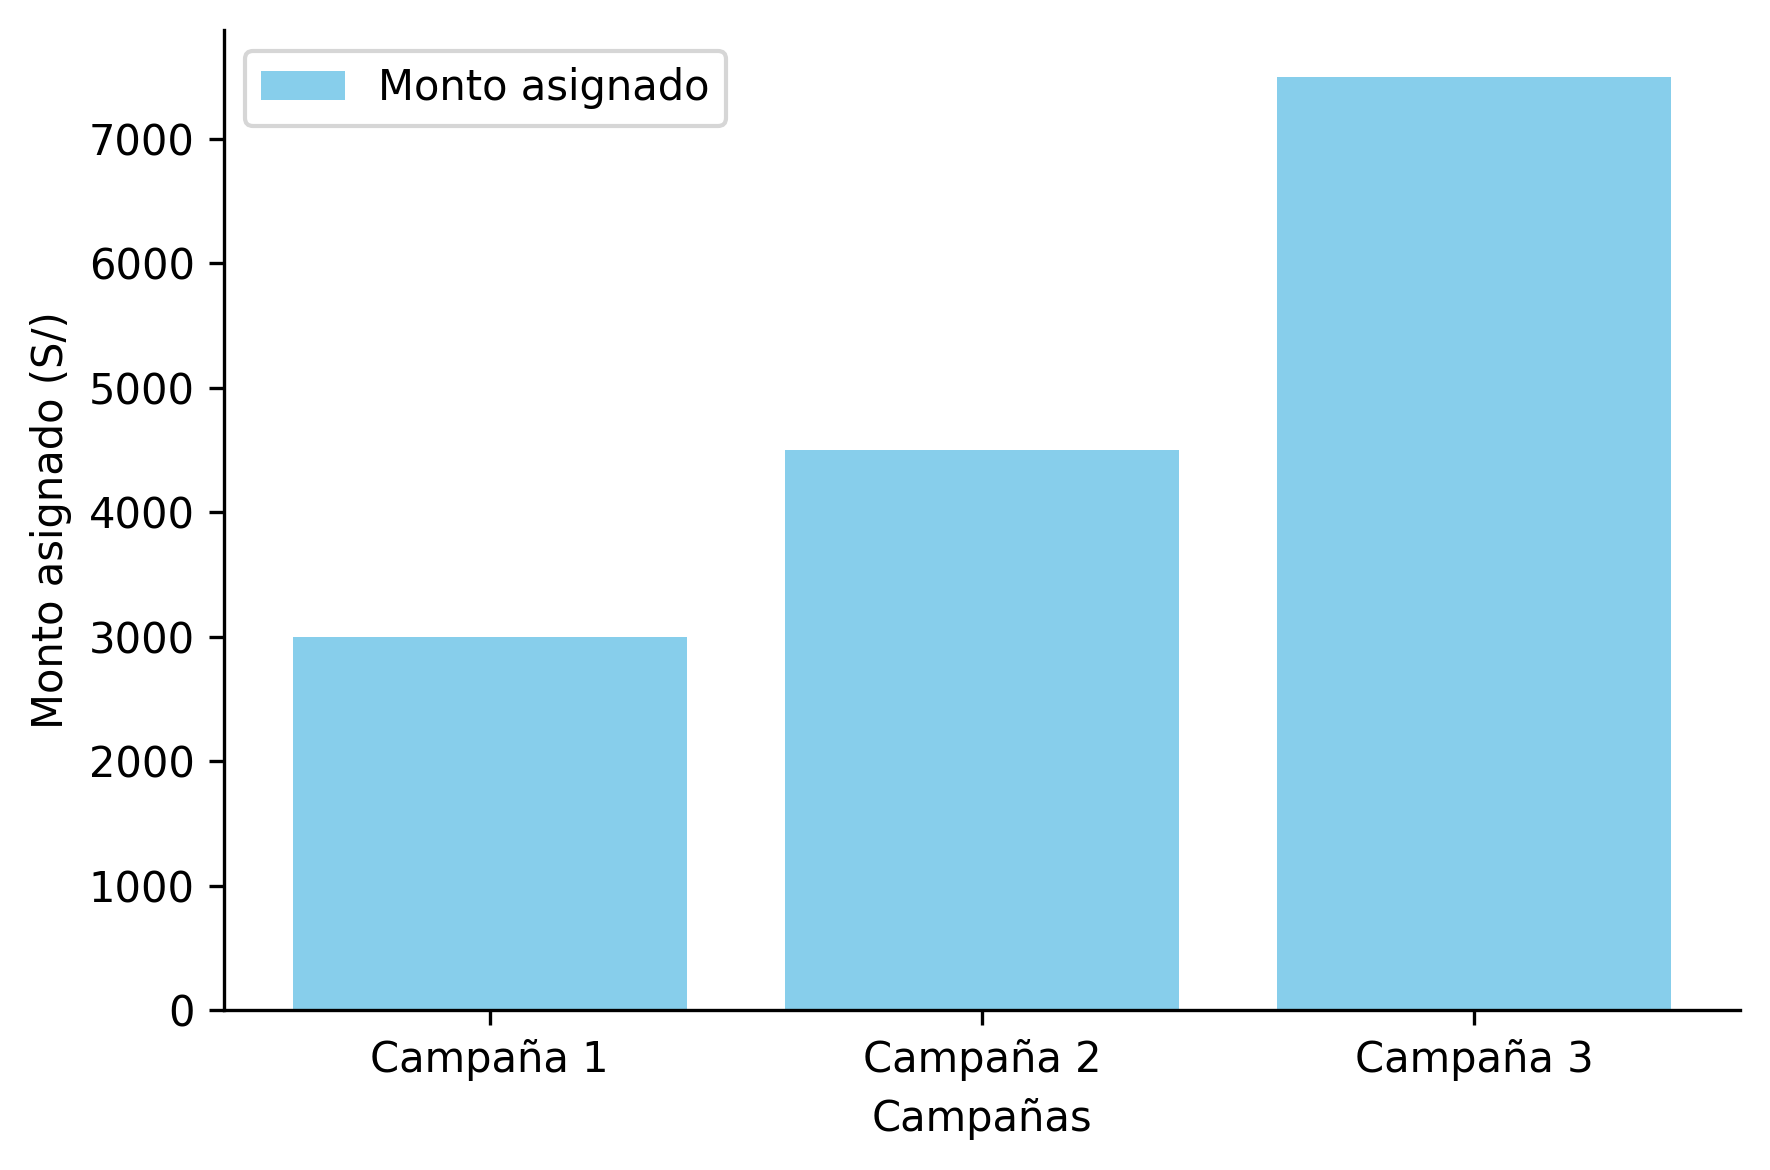
\includegraphics[keepaspectratio]{index_files/figure-pdf/cell-10-output-1.png}}

}

\end{figure}%

\subsection{Ejercicio 4}\label{ejercicio-4}

\textbf{Problema}: Un contrato de servicios tiene un costo original de
S/ 1,000. Se aplican dos descuentos sucesivos del 15\% y del 10\%. ¿Cuál
es el costo final después de los descuentos?

\textbf{Solución}:

Para calcular el costo final, usamos la fórmula de descuentos sucesivos
para encontrar el descuento único equivalente:

\[
\text{Descuento único} = (a + b) - \frac{a \cdot b}{100}
\]

Donde \(a = 15%
\) y \(b = 10%
\):

\[
\text{Descuento único} = (15 + 10) - \frac{15 \cdot 10}{100} = 25 - 1.5 = 23.5
\]

El descuento total es del 23.5\%. Calculamos el monto del descuento:

\[
\text{Monto descontado} = 23.5% \text{ de } 1,000 = \frac{23.5}{100} \cdot 1,000 = 235
\]

El costo final es:

\[
1,000 - 235 = 765
\]

El costo final es S/ 765.

\section{Conclusiones y
Recomendaciones}\label{conclusiones-y-recomendaciones}

La proporcionalidad, a través de herramientas como la regla de tres
simple, el reparto proporcional y los porcentajes, proporciona un marco
matemático para abordar desafíos en la gestión de recursos y el análisis
de datos. Estas técnicas permiten optimizar la asignación de
presupuestos, planificar tiempos de producción y evaluar métricas de
impacto, asegurando decisiones estratégicas basadas en cálculos
precisos. Su simplicidad y versatilidad las convierten en recursos
esenciales para profesionales que buscan eficiencia en entornos
dinámicos, conectando la teoría matemática con aplicaciones prácticas.

Para maximizar el impacto de estas herramientas, se recomienda
incorporar módulos prácticos en los planes de estudio de ciencias de la
comunicación, enfocados en resolver problemas reales, como la
distribución de recursos o el análisis de indicadores de audiencia.
Asimismo, se sugiere desarrollar talleres interactivos y recursos
digitales, como simuladores o aplicaciones, que faciliten el aprendizaje
de estas técnicas y refuercen las competencias cuantitativas de los
estudiantes.

\section{Bibliografía y
referencias}\label{bibliografuxeda-y-referencias}

\phantomsection\label{refs}
\begin{CSLReferences}{1}{0}
\bibitem[\citeproctext]{ref-abdounurPreliminarySurveyEmergence2009}
Abdounur, O. J. (2009). A Preliminary Survey on the Emergence of an
Arithmetical Theory of Ratios. \emph{Circumscribere}, \emph{9}, 1-8.
\url{https://repositorio.usp.br/item/003065271}

\bibitem[\citeproctext]{ref-aricanInvestigatingPreserviceMathematics2022}
Arican, M., \& Kiymaz, Y. (2022). Investigating {Preservice Mathematics
Teachers}' {Definitions}, {Formulas}, and {Graphs} of {Directly} and
{Inversely Proportional Relationships}. \emph{The Mathematics
Enthusiast}, \emph{19}(2), 632-656.
\url{https://doi.org/10.54870/1551-3440.1566}

\bibitem[\citeproctext]{ref-kimSilvioBellisRatio2023}
Kim, W. (2023). Silvio {Belli}'s {On Ratio} and {Proportion} \textbar{}
{Nexus Network Journal}. \emph{Nexus Network Journal}, \emph{25}, 5-39.
\url{https://doi.org/10.1007/s00004-022-00638-4}

\bibitem[\citeproctext]{ref-parkHistoricalDevelopmentsProcess2008}
Park, J.-S. (2008). The Historical Developments Process of the
Representations and Meanings for Ratio and Proportion. \emph{Journal for
History of Mathematics}, \emph{21}(3), 53-66.
\url{https://koreascience.kr/article/JAKO200800557082829.page}

\bibitem[\citeproctext]{ref-thorupPreeuclideanTheoryProportions1992}
Thorup, A. (1992). A Pre-Euclidean Theory of Proportions. \emph{Archive
for History of Exact Sciences}, \emph{45}(1), 1-16.
\url{https://doi.org/10.1007/BF00375885}

\end{CSLReferences}






\end{document}
